% Tikz plot for UQ. This is based on the tikz code of
% Fabian Schuh for the tikz examples website
\documentclass[10pt,final,xcolor=dvipsnames]{beamer}
%\usepackage{etex}

\usetheme{Madrid}

\usepackage{xspace}
%\usepackage{enumitem}
\usepackage[mathscr]{euscript}
\usepackage{subfigure}
\hypersetup{colorlinks,linkcolor=,urlcolor=blue}

% \usetheme{Boadilla}
% \usecolortheme{seahorse}

% the macros, packages, etc:
\usepackage[absolute,overlay]{textpos}
\setbeamertemplate{items}[ball]
\setbeamertemplate{blocks}[rounded][shadow=true]
\setbeamertemplate{navigation symbols}{}
\newenvironment{reference}[2]{%
  \begin{textblock*}{\textwidth}(#1,#2)
  \scriptsize{\it\color{black}}}{\end{textblock*}}
\setbeamertemplate{blocks}[rounded]% [shadow=false]
\newenvironment{boxalertenv}{\begin{altenv}%
      {\usebeamertemplate{alerted text begin}\usebeamercolor[fg]{alerted text}\usebeamerfont{alerted text}\colorbox{bg}}
      {\usebeamertemplate{alerted text end}}{\color{.}}{}}{\end{altenv}}

\newcommand{\tcmag}[1]{\textcolor{magenta}{{#1}}}
\usepackage{graphicx}
\usepackage{multirow,color}
\usepackage{bbm}
\usepackage{amsfonts,amsmath,amssymb,amsbsy,amsthm}
\usepackage{movie15}
\usepackage{arydshln}

\makeatletter
\renewcommand*\env@matrix[1][*\c@MaxMatrixCols c]{%
  \hskip -\arraycolsep
  \let\@ifnextchar\new@ifnextchar
  \array{#1}}

%\usepackage{movie15}
%\usepackage{multimedia}
% custom commands (add your own macros here)

\definecolor{bronze}{rgb}{0.8, 0.5, 0.2}
\definecolor{goldenyellow}{rgb}{1.0, 0.87, 0.0}
\definecolor{amber}{rgb}{1.0, 0.75, 0.0}
\definecolor{azure}{rgb}{0.94, 1.0, 1.0}
\definecolor{bittersweet}{rgb}{1.0, 0.44, 0.37}
\definecolor{brass}{rgb}{0.71, 0.65, 0.26}
\definecolor{camel}{rgb}{0.76, 0.6, 0.42}
\setbeamercolor{block body}{bg=camel!30}
\usefonttheme[onlymath]{serif}
\usepackage{color}

\usepackage{amsmath}
\usepackage{mathtools}
\usepackage{tikz}
\usepackage{amsfonts,amsmath,amssymb,amsbsy,amsthm}
%\usecolortheme{tango}

%\usefonttheme{serif}     % Font theme: serif
%\usefonttheme[stillsansseriftext]{serif} 
%\renewcommand*\familydefault{\sfdefault}

\usepackage{pgf}
%\usepackage{pgfplots}
\usepackage{amssymb}
\usepackage{amsmath}
\usepackage{tikz}
\usepackage{verbatim}
%\usepackage{movie15}
\usepackage{tikz,pgfplots}

%\usepackage[active,tightpage]{preview}
%\PreviewEnvironment{tikzpicture}
\usetikzlibrary{arrows,automata}
\usetikzlibrary{positioning}
\usetikzlibrary{fit}

%\input{ccgodef}
\newcommand{\iparb}{\bar{\ipar}}
\newcommand{\euclidnorm}[1]{\left\| {#1} \right\|_2}
\newcommand{\incu}{\upupsilon}
\newcommand{\incp}{\uprho}
\newcommand{\QoIquad}{\QoI_\text{quad}}
\newcommand{\tcblue}[1]{\textcolor{blue}{#1}}

%%%%%%%%%%%%%%%%%%%%%%%%%%%%%%%%%%%%%%%%%%%%%%%%%%%%%%
%% this def file is based on the ccgodef
%%%%%%%%%%%%%%%%%%%%%%%%%%%%%%%%%%%%%%%%%%%%%%%%%%%%%
% packages
%\usepackage{booktabs}
%\usepackage[mathscr]{euscript}
%\usepackage{color}
%% mathdesgin or ams
%%\usepackage{amssymb,mathrsfs}
%\usepackage{graphicx}
%\usepackage{algorithmic,algorithm}
%\usepackage{tikz,pgfplots}
%\usepackage{upgreek}
%%\usepackage{showkeys,cite}
%\usepackage{multirow}
%\usepackage{yfonts}
%\usepackage{mathtools}
%\usepackage[normalem]{ulem}
%\usepackage{latexsym}
%\usepackage{url}
%\usepackage{amsmath,amssymb,amsbsy,amsfonts}
%\usepackage{enumitem}

\newcommand{\zapspace}{\topsep=0pt\partopsep=0pt\itemsep=0pt\parskip=0pt}

%% Notice macros
%\newcommand{\notice}[1]{\textcolor{Chameleon3}{#1}}
%\newcommand{\Notice}[1]{\textcolor{ScarletRed2}{#1}}
%\newcommand{\nnote}[1]{\noindent\emph{\textcolor{grass}{N: #1\,}}}
%\newcommand{\unote}[1]{\noindent\emph{\textcolor{blue}{U: #1\,}}}
%\newcommand{\onote}[1]{\noindent\emph{\textcolor{red}{O: #1\,}}}
%
%% colors
%\definecolor{utorange}{rgb}{0.8,0.33,0.}
%\definecolor{themec}{RGB}{51,108,121}
%\definecolor{darkred}{rgb}{.6,.1,.1}
%\definecolor{darkblue}{rgb}{.1,.1,.9}
%\definecolor{greenback}{rgb}{.19,.94,.13}
%\definecolor{orange}{rgb}{.76,.39,.13}
%\definecolor{grass}{rgb}{.19,.64,.13}
%\definecolor{sierp}{RGB}{209,28,209}
%\definecolor{bgorange}{rgb}{1.,.95,.78}
%\definecolor{grassgreen}{RGB}{92,135,39}
%\definecolor{thinbox}{rgb}{.7,.8,1.}

% general
\newcommand{\defeq}{\vcentcolon=}
%\newcommand{\del}[2]{\frac{\partial{#1}}{\partial{#2}}}
\renewcommand{\vec}[1]{{\mathchoice
                     {\mbox{\boldmath$\displaystyle{#1}$}}
                     {\mbox{\boldmath$\textstyle{#1}$}}
                     {\mbox{\boldmath$\scriptstyle{#1}$}}
                     {\mbox{\boldmath$\scriptscriptstyle{#1}$}}}}
\renewcommand{\ker}{\mathsf{ker}}
\newcommand{\ran}{\mathsf{range}}
\newcommand{\dom}{\mathsf{dom}}
\newcommand{\trace}{\mathsf{tr}}
\newcommand{\eps}{\varepsilon}
%\newcommand{\norm}[1]{\left\| {#1} \right\|}
\newcommand{\ip}[2]{{\left\langle {#1}, {#2} \right\rangle}}
\newcommand{\mip}[2]{\left\langle{#1}, {#2}\right\rangle_{\!\scriptscriptstyle{\text{M}}}}
\newcommand{\mat}[1]{\mathbf{{#1}}}
\newcommand\restr[2]{{
  \left.\kern-\nulldelimiterspace % automatically resize the bar with \right
  {#1}\vphantom{\big|} \right|_{#2}}}
\newcommand{\angles}[1]{\left\langle #1 \right\rangle}

% sets of numbers
\newcommand{\R}{\mathbb{R}}
\newcommand{\Z}{\mathbb{Z}}
\newcommand{\N}{\mathbb{N}}

\newcommand{\BB}{\mat{B}}
\newcommand{\Amat}{\mat{A}}
\newcommand{\VV}{\mat{V}}
\newcommand{\RR}{\mat{R}}

% commonly used mathcals
\newcommand{\A}{\mathcal{A}}
\newcommand{\B}{\mathcal{B}}
\newcommand{\C}{\mathcal{C}}
\newcommand{\D}{\mathcal{D}}
\newcommand{\E}{\mathcal{E}}
\newcommand{\F}{\mathcal{F}}
\newcommand{\G}{\mathcal{G}}
\newcommand{\J}{\mathcal{J}}
\newcommand{\U}{\mathcal{U}}
\newcommand{\Reg}{\mathcal{R}}

% shorthands
\newcommand{\bit}{\begin{itemize}}
\newcommand{\eit}{\end{itemize}}
\newcommand{\bdm} {\begin{displaymath}}
\newcommand{\edm} {\end{displaymath}}

% Probability (general)
\newcommand{\prob}{\mathsf{Prob}}
\newcommand{\borel}{\mathscr{B}}
\newcommand{\ave}{\mathsf{E}}
\newcommand{\GM}[2]{\mathcal{N}\!\left( {#1}, {#2}\right)}

% Bayesian stuff

\newcommand{\noisem}{\mu_{\text{noise}}}
\newcommand{\obs}{\vec{d}}
\newcommand{\ipar}{m}

\newcommand{\iparpr}{m_{\text{pr}}}
\newcommand{\iparref}{m_{\text{ref}}}
\newcommand{\iparmap}{m_{\scriptscriptstyle\text{MAP}}}
\newcommand{\dpar}{\vec{m}}
\newcommand{\dparmap}{\vec{m}_{\scriptscriptstyle\text{MAP}}}
%\newcommand{\priorm}{\mu_{\text{pr}}}
%\newcommand{\postm}{\mu_{\text{post}}}
\newcommand{\M}{\mat{M}}% the Mass matrix
%\newcommand{\ff}{\vec{f}}     % parameter-to-obs MAP
\newcommand{\ff}{\mathcal{F}} % parameter-to-obs MAP
\newcommand{\aff}{\tilde{\mathcal{F}}} % parameter-to-obs MAP
\newcommand{\noise}{\bs e}
\newcommand{\observables}{\bs d}
\newcommand{\data}{ \observables_{\rm{obs}} }
\newcommand{\uobs}{ \uu_{\rm{obs}} }
\newcommand{\datacomponent}[1]{ \observables_{\rm{obs}}^{#1} }
\newcommand{\FF}{{\ensuremath{\mat{F}}}}
\newcommand{\W}{{\ensuremath{\mat{W}}}}
\newcommand{\I}{{\ensuremath{\mat{I}}}}

\newcommand{\prior} {\pi_{\mbox{\tiny prior}}}
\newcommand{\like}{\pi_{\mbox{\tiny like}}}
\newcommand{\piobs}{\pi_{\mbox{\tiny obs}}}
\newcommand{\post}{\pi_{\mbox{\tiny post}}}
\newcommand{\pinoise}{\pi_{\mbox{\tiny noise}}}

\newcommand{\mupost}{\mu_{\mbox{\tiny post}}}
\newcommand{\muprior}{\mu_{\mbox{\tiny prior}}}

\newcommand{\ncov} {\bs{\Gamma}_{\!\mbox{\tiny noise}} }
\newcommand{\prcov} {\bs{\Gamma}_{\!\mbox{\tiny prior}} }
\newcommand{\postcov} {\bs{\Gamma}_{\!\mbox{\tiny post}} }
\newcommand{\aFF}{{\tilde{\ensuremath{\mat{F}}}}}
\newcommand{\ncovw} {\bs{W}}
\newcommand{\prcovr} {\bs{R}}

\newcommand{\Cprior}{\mathcal{C}_{\text{\tiny{prior}}}}
\newcommand{\Cpost}{\mathcal{C}_{\text{\tiny{post}}}}

\newcommand{\map} {{m}_{\mbox{\tiny MAP}} }
\newcommand{\dmap} {{\vec{m}}_{\mbox{\tiny MAP}} }
\newcommand{\mpr} {{\vec{m}}_{\mbox{\tiny pr}} }
\newcommand{\dbeta}{\vec{\beta}}
\newcommand{\dn}{\vec{n}}



\newcommand{\Hpost}  { \bs H }
\newcommand{\Hmisfit}{ \mat{H}_{\mbox{\tiny misfit}} }
\newcommand{\tHmisfit}{\tilde{\mat{H}}_{\mbox{\tiny misfit}} }
\newcommand{\HT}{\matrix{\tilde{H}}_{\mbox{\tiny misfit}}}
\newcommand{\HTinf}{\tilde{H}_{\text{misfit}}}
\newcommand{\Vr} {\bs V_r}
\newcommand{\Dr} {\bs D_r}
\newcommand{\Ir} {\bs I_r}

%\newcommand{\Ge}{ \ensuremath{\matrix{G}}_{\!\mbox{\tiny e}}}
%\newcommand{\Op}{ \ensuremath{\matrix{O}}_{\!\mbox{\tiny p}}}
\newcommand{\Ge}{ \mathcal{G}_{\!\mbox{\tiny e}}}
\newcommand{\Op}{ \mathcal{O}_{\!\mbox{\tiny p}}}
\newcommand{\HH}{ \ensuremath{\matrix{H}} }
\newcommand{\SI}{ \ensuremath{{\Sigma}} }
\newcommand{\PP}{ \ensuremath{\matrix{\Psi}} }
%\newcommand{\WW}{ \ensuremath{\matrix{W}} }
\newcommand{\WW}{ \mathcal{W}}

% Macros for three different forms of adjoint operator
\newcommand{\adjMacroMM}[1]{{#1}^*}
\newcommand{\adjMacroME}[1]{{#1}^\natural}
\newcommand{\adjMacroEM}[1]{{#1}^\diamond}
\newcommand{\adjMacroEMINV}[1]{{#1}^{-\diamond}}
\newcommand{\Aadj}{\adjMacroMM{\A}}
\newcommand{\Badj}{\adjMacroMM{\BB}}
\newcommand{\iFadj}{\adjMacroME{\iF}}
\newcommand{\Fadj}{\adjMacroME{\F}}
\newcommand{\Vadj}{\adjMacroEM{\VV}}
\newcommand{\Ladj}{\adjMacroEM{\L}}

\def\bfG{\mbox{\boldmath$G$}}
\newcommand{\mc}[1]{\mathcal{#1}}

%%%%%%%%%%%%%%%%%%%%%%%%%%%%%%%%%%%%
% custom commands to the sc14 paper
%%%%%%%%%%%%%%%%%%%%%%%%%%%%%%%%%%%%
\newcommand{\SNR}{\ensuremath{\text{SNR}}}

\newcommand{\gbf}[1]{\boldsymbol{#1}}
\newcommand{\bs}[1]{\ensuremath{\boldsymbol{#1}}}

\newcommand{\edot}{\dot{\gbf{\varepsilon}}}
\newcommand{\edotsec}{\edot_\mathrm{II}}
\newcommand{\secinve}{\edot_\mathrm{II}}

\DeclareMathOperator{\sym}{sym}
%\DeclareMathOperator{\trace}{tr}
%\DeclareMathOperator{\diag}{diag}

\newcommand{\Div}{\mbox{div}}
\newcommand{\Grad}{{\bf \nabla}}
\newcommand{\grad}{\nabla}

\newcommand{\pt}{\tilde{p}}
\newcommand{\vt}{\tilde{\vv}}
\newcommand{\qt}{\tilde{q}}
\newcommand{\betat}{\tilde{\beta}}

\newcommand{\uh}{\hat{\uu}}
\newcommand{\ph}{\hat{p}}
\newcommand{\vh}{\hat{\vv}}
\newcommand{\qh}{\hat{q}}
\newcommand{\betah}{\hat{\beta}}

\renewcommand{\vec}[1]{\gbf{#1}}
\newcommand{\cvec}[1]{{#1}}

\newcommand{\uu}{\ensuremath{\vec{u}}}
\newcommand{\vv}{\ensuremath{\vec{v}}}

\definecolor{darkblue}{rgb}{.1,.1,.9}
\definecolor{utorange}{rgb}{0.8,0.33,0.}
% this are only needed for presentations
\newcommand{\tcb}[1]{\textcolor{blue}{{#1}}}
\newcommand{\tcdb}[1]{\textcolor{utorange}{{#1}}}
\newcommand{\tcr}[1]{\ensuremath{\textcolor{red}{{#1}}}}
\newcommand{\tcdr}[1]{\textcolor{darkred}{{#1}}}
\newcommand{\tcm}[1]{\textcolor{ForestGreen}{{#1}}}
\newcommand{\tcmag}[1]{\textcolor{magenta}{{#1}}}
\newcommand{\tco}[1]{\textcolor{VioletRed}{{#1}}}
\newcommand{\tcc}[1]{\textcolor{cyan}{{#1}}}
\newcommand{\dg}[1]{\textcolor{black!65!green}{{#1}}}
\newcommand{\tcg}[1]{\textcolor{blue!70!black!30!green}{{#1}}}
\newcommand{\tcdg}[1]{\textcolor{blue!20!black!50!green}{{#1}}}
\newcommand{\tcch}[1]{\textcolor{cyan}{\hat{{#1}}}}
\newcommand{\tcmhb}[1]{\textcolor{magenta}{\hat{\gbf{{#1}}}}}
\newcommand{\tcmh}[1]{\textcolor{magenta}{\hat{{#1}}}}
\newcommand{\tcbb}[1]{\textcolor{blue}{\gbf{{#1}}}}
\newcommand{\tcgb}[1]{\textcolor{grass}{\gbf{{#1}}}}
\newcommand{\tcct}[1]{\textcolor{cyan}{\tilde{{#1}}}}
\newcommand{\tcmtb}[1]{\textcolor{magenta}{\tilde{\gbf{{#1}}}}}
\newcommand{\tcmt}[1]{\textcolor{magenta}{\tilde{{#1}}}}
\newcommand{\tcotb}[1]{\textcolor{utorange}{\tilde{\gbf{{#1}}}}}
\newcommand{\tcot}[1]{\textcolor{utorange}{\tilde{{#1}}}}
\newcommand{\tcohb}[1]{\textcolor{utorange}{\hat{\gbf{{#1}}}}}
\newcommand{\tcoh}[1]{\textcolor{utorange}{\hat{{#1}}}}

\renewcommand{\matrix}[1] {\ensuremath{\boldsymbol{#1}}}

\newcommand{\bndFS}{\Gamma_{\!\mbox{\scriptsize $FS$}}}
\newcommand{\bndB}{\Gamma_{\!\mbox{\scriptsize $B$}}}
\newcommand{\bndT}{\Gamma_{\!\mbox{\scriptsize $T$}}}

\usepackage{xspace}
\newcommand{\software}[1]{\texttt{#1}\xspace}
\newcommand{\hip}{\texttt{hIPPYlib}\xspace}
\newcommand{\bhip}{\texttt{{\bf hIPPYlib}}\xspace}
\newcommand{\Fe}{\texttt{FEniCS}\xspace}
\newcommand{\pet}{\texttt{PETSc}\xspace}


\newcommand{\del}{\partial}
%\newcommand{\D}{\mathcal{D}}
\newcommand{\Ns}{{N_s}}
\newcommand{\Ntau}{{N_{\tau}}}
\newcommand{\iFF}{\mathcal{F}}
%\newcommand{\priorm}{\muprior}
\newcommand{\Acal}{\mc{A}}
%\newcommand{\postm}{\mupost}
\newcommand{\iparpost}{\ipar_\text{post}}
\newcommand{\dd}{\vec{\bar{d}}}
\newcommand{\obsop}{\mathcal{B}}

\newcommand{\GN}{\ensuremath{\Gamma_{\!\!N}}}
\newcommand{\Exp}[1]{e^{{#1}}}
\newcommand{\GD}{\ensuremath{\Gamma_{\!\!D}}}
\newcommand{\Vg}{\mathscr{V}_{\!g}}
\newcommand{\V}{\mathscr{V}_{\!\scriptscriptstyle{0}}}
\newcommand{\eip}[2]{\left\langle{#1}, {#2}\right\rangle_{\!{\R^q}}}
\newcommand{\Wn}{\mat{W}_{\!\sigma}}
\newcommand{\cip}[2]{\left\langle{#1}, {#2}\right\rangle_{\!\CM}}
\newcommand{\CM}{\mathscr{E}}
\newcommand{\LI}{\mathscr{L}}
\renewcommand{\H}{\mathcal{H}}
\newcommand{\Nd}{{n_{\text{d}}}}
\newcommand{\Ntr}{{n_{\text{tr}}}}
\newcommand{\ipart}{m_{\scriptscriptstyle\text{true}}}
\newcommand{\ut}[1]{\ensuremath{\tilde{#1}}}

\newcommand{\LRp}[1]{\left( #1 \right)}
\newcommand{\LRs}[1]{\left[ #1 \right]}
\newcommand{\LRa}[1]{\left< #1 \right>}
\newcommand{\LRc}[1]{\left\{ #1 \right\}}

\newcommand{\xx}{\ensuremath{\boldsymbol x}}
\newcommand{\rr}{\ensuremath{\boldsymbol r}}
\newcommand{\e}{\ensuremath{\boldsymbol e}}
\newcommand{\x}{\xx}
\newcommand{\y}{\ensuremath{\boldsymbol y}}
\newcommand{\z}{\ensuremath{\boldsymbol z}}
\renewcommand{\r}{\ensuremath{\boldsymbol r}}
\newcommand{\s}{\ensuremath{\boldsymbol s}}

\newcommand{\hilb}{\mathscr{H}}
\newcommand{\half} {\ensuremath{\frac{1}{2}}}
\newcommand{\nor}[1]{\left\| #1 \right\|}
\newcommand{\equaldef}{{:=}}
\newcommand{\iFFadj}{\adjMacroMM{\iFF}}

\newcommand{\istate}{u}
\newcommand{\iparspace}{\mathcal{M}}
\newcommand{\iadj}{p}
\DeclareMathOperator*{\argmin}{argmin} 
\DeclareMathOperator{\diag}{diag} 


\newcommand{\err}{\vec{\eta}}
\newcommand{\beps}{\bs{\eps}}
\newcommand{\bbeps}{\bar{\bs{\eps}}}
\newcommand{\bnu}{\bs{\nu}}
\newcommand{\ncovbeps} {\bs{\Gamma}_{\!\mbox{\tiny \beps}} }
\newcommand{\ncovbnu} {\bs{\Gamma}_{\!\mbox{\tiny \bnu}} }
\newcommand{\norm}[2][]{\left\Vert #2\right\Vert_{#1}}
\newcommand{\dbetamap}{\vec{\beta}_{\scriptscriptstyle\text{MAP}}}
\newcommand{\betamap}{{\beta}_{\scriptscriptstyle\text{MAP}}}
\newcommand{\smallB}{\scriptscriptstyle\text{B}}
\definecolor{lightblue}{cmyk}{0.88,0.44,0,0.07}
\newcommand{\betapr}{\beta_{\text{pr}}}
\newcommand{\ntrue}{a_{\scriptscriptstyle\text{true}}}
\newcommand{\NoiseForcing}{\xi}
\newcommand{\ProbMeasClass}{\mathcal{P}}
\newcommand{\ProbMeas}{\mathbbm{P}}
\newcommand{\SigmaAlg}{F}

\newcommand{\Hmatrix}{\bs{H}}

\tikzset{
    state/.style={
           rectangle,
           rounded corners,
           draw=black, very thick,
           minimum height=3em,
           inner sep=1pt,
           text centered,
           },
}

%
\newcommand{\zapspace}{\topsep=0pt\partopsep=0pt\itemsep=0pt\parskip=0pt}

%
\newcommand{\notice}[1]{\textcolor{Chameleon3}{#1}}
\newcommand{\Notice}[1]{\textcolor{ScarletRed2}{#1}}
\newcommand{\nnote}[1]{\noindent\emph{\textcolor{grass}{N: #1\,}}}
\newcommand{\emil}[1]{\noindent\emph{\textcolor{blue}{Emil: #1\,}}}
\newcommand{\julie}[1]{\noindent\emph{\textcolor{red}{Julie: #1\,}}}
\newcommand{\unote}[1]{\noindent\emph{\textcolor{blue}{U: #1\,}}}
\newcommand{\onote}[1]{\noindent\emph{\textcolor{red}{O: #1\,}}}
\definecolor{mygreen}{rgb}{0.5,0.05,0.15}
\newcommand{\cosmin}[1]{\noindent\emph{\textcolor{mygreen}{#1\,}}}

%
\definecolor{utorange}{rgb}{0.8,0.33,0.}
\definecolor{themec}{RGB}{51,108,121}
\definecolor{darkred}{rgb}{.6,.1,.1}
\definecolor{darkblue}{rgb}{.1,.1,.9}
\definecolor{greenback}{rgb}{.19,.94,.13}
\definecolor{orange}{rgb}{.76,.39,.13}
\definecolor{grass}{rgb}{.19,.64,.13}
\definecolor{sierp}{RGB}{209,28,209}
\definecolor{bgorange}{rgb}{1.,.95,.78}
\definecolor{grassgreen}{RGB}{92,135,39}
\definecolor{thinbox}{rgb}{.7,.8,1.}

%
\newcommand{\defeq}{\vcentcolon=}
%
\renewcommand{\vec}[1]{{\mathchoice
                     {\mbox{\boldmath$\displaystyle{#1}$}}
                     {\mbox{\boldmath$\textstyle{#1}$}}
                     {\mbox{\boldmath$\scriptstyle{#1}$}}
                     {\mbox{\boldmath$\scriptscriptstyle{#1}$}}}}
\renewcommand{\ker}{\mathsf{ker}}
\newcommand{\ran}{\mathsf{range}}
\newcommand{\dom}{\mathsf{dom}}
\newcommand{\trace}{\mathsf{tr}}
\newcommand{\eps}{\varepsilon}
\newcommand{\norm}[1]{\left\| {#1} \right\|}
\newcommand{\ip}[2]{{\left\langle {#1}, {#2} \right\rangle}}
\newcommand{\mip}[2]{\left\langle{#1}, {#2}\right\rangle_{\!\scriptscriptstyle{\text{M}}}}
\newcommand{\mat}[1]{\mathbf{{#1}}}
\newcommand\restr[2]{{
  \left.\kern-\nulldelimiterspace %
  {#1}\vphantom{\big|} \right|_{#2}}}
\newcommand{\angles}[1]{\left\langle #1 \right\rangle}

%
\newcommand{\R}{\mathbb{R}}
\newcommand{\Z}{\mathbb{Z}}
\newcommand{\N}{\mathbb{N}}

\newcommand{\BB}{\mat{B}}
\newcommand{\Amat}{\mat{A}}
\newcommand{\VV}{\mat{V}}
\newcommand{\RR}{\mat{R}}

%
\newcommand{\A}{\mathcal{A}}
\newcommand{\B}{\mathcal{B}}
\newcommand{\C}{\mathcal{C}}
\newcommand{\D}{\mathcal{D}}
\newcommand{\E}{\mathcal{E}}
\newcommand{\F}{\mathcal{F}}
\newcommand{\G}{\mathcal{G}}
\newcommand{\J}{\mathcal{J}}
\newcommand{\U}{\mathcal{U}}
\newcommand{\Reg}{\mathcal{R}}

%
\newcommand{\bit}{\begin{itemize}}
\newcommand{\eit}{\end{itemize}}
\newcommand{\bdm} {\begin{displaymath}}
\newcommand{\edm} {\end{displaymath}}

%
\newcommand{\prob}{\mathsf{Prob}}
\newcommand{\borel}{\mathscr{B}}
\newcommand{\ProbMeasClass}{\mathcal{P}}
\newcommand{\ProbMeas}{\mathbbm{P}}
\newcommand{\SigmaAlg}{F}
\newcommand{\ave}{\mathsf{E}}
\newcommand{\GM}[2]{\mathcal{N}\!\left( {#1}, {#2}\right)}

%
\newcommand{\NoiseForcing}{\xi}
\newcommand{\noisem}{\mu_{\text{noise}}}
\newcommand{\obs}{\F}%
\newcommand{\dobs}{{\vec{d}}}
\newcommand{\obsT}{{\vec{d}_{\scriptscriptstyle\text{obs}}}}
\newcommand{\ipar}{m}
\newcommand{\iparT}{m_{\mathrm T}}
\newcommand{\iparpr}{m_{\text{prior}}}
\newcommand{\iparmap}{m_{\scriptscriptstyle\text{MAP}}}
\newcommand{\dpar}{\vec{m}}
\newcommand{\dparmap}{\vec{m}_{\scriptscriptstyle\text{MAP}}}
%
%
\newcommand{\M}{\mat{M}}%
%
\newcommand{\ff}{\mathcal{F}} %
\newcommand{\noise}{\bs e}
\newcommand{\observables}{\bs d}
\newcommand{\data}{ \observables_{\rm{obs}} }
\newcommand{\uobs}{ \uu_{\rm{obs}} }
\newcommand{\datacomponent}[1]{ \observables_{\rm{obs}}^{#1} }
\newcommand{\FF}{{\ensuremath{\mat{F}}}}
\newcommand{\W}{{\ensuremath{\mat{W}}}}
\newcommand{\I}{{\ensuremath{\mat{I}}}}
\newcommand{\ScoreFcn}{S}
\newcommand{\Nobs}{M}
\newcommand{\Expectation}{\mathbb{E}}


\newcommand{\prior} {\pi_{\mbox{\tiny prior}}}
\newcommand{\like}{\pi_{\mbox{\tiny like}}}
\newcommand{\piobs}{\pi_{\mbox{\tiny obs}}}
\newcommand{\pinoise}{\pi_{\mbox{\tiny $\xi$}}}
\newcommand{\post}{\pi_{\mbox{\tiny post}}}

\newcommand{\mupost}{\mu_{\mbox{\tiny post}}}
\newcommand{\muprior}{\mu_{\mbox{\tiny prior}}}

\newcommand{\ncov} {\bs{\Gamma}_{\!\mbox{\tiny noise}} }
\newcommand{\prcov} {\bs{\Gamma}_{\!\mbox{\tiny prior}} }
\newcommand{\postcov} {\bs{\Gamma}_{\!\mbox{\tiny post}} }

\newcommand{\Cprior}{\mathcal{C}_{\text{\tiny{prior}}}}
\newcommand{\Cpost}{\mathcal{C}_{\text{\tiny{post}}}}

\newcommand{\map} {{m}_{\mbox{\tiny MAP}} }
\newcommand{\dmap} {{\vec{m}}_{\mbox{\tiny MAP}} }
\newcommand{\mpr} {{\vec{m}}_{\mbox{\tiny pr}} }
\newcommand{\dbeta}{\vec{m}}

\newcommand{\Hpost}  { \bs H }
\newcommand{\Hmisfit}{ \mat{H}_{\mbox{\tiny misfit}} }
\newcommand{\tHmisfit}{\tilde{\mat{H}}_{\mbox{\tiny misfit}} }
\newcommand{\HT}{\matrix{\tilde{H}}_{\mbox{\tiny misfit}}}
\newcommand{\HTinf}{\tilde{H}_{\text{misfit}}}
\newcommand{\Vr} {\bs V_r}
\newcommand{\Dr} {\bs D_r}
\newcommand{\Ir} {\bs I_r}

%
%
\newcommand{\Ge}{ \mathcal{G}_{\!\mbox{\tiny e}}}
\newcommand{\Op}{ \mathcal{O}_{\!\mbox{\tiny p}}}
\newcommand{\HH}{ \ensuremath{\matrix{H}} }
\newcommand{\SI}{ \ensuremath{{\Sigma}} }
\newcommand{\PP}{ \ensuremath{\matrix{\Psi}} }
%
\newcommand{\WW}{ \mathcal{W}}

%
\newcommand{\adjMacroMM}[1]{{#1}^*}
\newcommand{\adjMacroME}[1]{{#1}^\natural}
\newcommand{\adjMacroEM}[1]{{#1}^\diamond}
\newcommand{\adjMacroEMINV}[1]{{#1}^{-\diamond}}
\newcommand{\Aadj}{\adjMacroMM{\A}}
\newcommand{\Badj}{\adjMacroMM{\BB}}
\newcommand{\iFadj}{\adjMacroME{\iF}}
\newcommand{\Fadj}{\adjMacroME{\F}}
\newcommand{\Vadj}{\adjMacroEM{\VV}}
\newcommand{\Ladj}{\adjMacroEM{\L}}

\def\bfG{\mbox{\boldmath$G$}}
\newcommand{\mc}[1]{\mathcal{#1}}

%
%
%
\newcommand{\SNR}{\ensuremath{\text{SNR}}}

\newcommand{\gbf}[1]{\boldsymbol{#1}}
\newcommand{\bs}[1]{\ensuremath{\boldsymbol{#1}}}

\newcommand{\edot}{\dot{\gbf{\varepsilon}}}
\newcommand{\edotsec}{\edot_\mathrm{II}}
\newcommand{\secinve}{\edot_\mathrm{II}}

\DeclareMathOperator{\sym}{sym}
%
%

\newcommand{\Div}{\mbox{div}}
\newcommand{\Grad}{{\bf \nabla}}

\newcommand{\pt}{\tilde{p}}
\newcommand{\vt}{\tilde{\vv}}
\newcommand{\qt}{\tilde{q}}
\newcommand{\betat}{\tilde{\beta}}

\newcommand{\uh}{\hat{\uu}}
\newcommand{\ph}{\hat{p}}
\newcommand{\vh}{\hat{\vv}}
\newcommand{\qh}{\hat{q}}
\newcommand{\betah}{\hat{\beta}}

\newcommand{\permeab}{\mathrm{m}}

\renewcommand{\vec}[1]{\gbf{#1}}
\newcommand{\cvec}[1]{{#1}}

\newcommand{\uu}{\ensuremath{\vec{u}}}
\newcommand{\vv}{\ensuremath{\vec{v}}}

\newcommand{\tcb}[1]{\textcolor{blue}{{#1}}}
\newcommand{\tcdb}[1]{\textcolor{darkblue}{{#1}}}
\newcommand{\tcr}[1]{\ensuremath{\textcolor{red}{{#1}}}}
\newcommand{\tcdr}[1]{\textcolor{darkred}{{#1}}}
\newcommand{\tcm}[1]{\textcolor{ForestGreen}{{#1}}}
\newcommand{\tco}[1]{\textcolor{VioletRed}{{#1}}}
\newcommand{\tcc}[1]{\textcolor{cyan}{{#1}}}
\newcommand{\dg}[1]{\textcolor{black!65!green}{{#1}}}
\newcommand{\tcg}[1]{\textcolor{blue!70!black!30!green}{{#1}}}
\newcommand{\tcdg}[1]{\textcolor{blue!20!black!50!green}{{#1}}}
\newcommand{\tcch}[1]{\textcolor{cyan}{\hat{{#1}}}}
\newcommand{\tcmhb}[1]{\textcolor{magenta}{\hat{\gbf{{#1}}}}}
\newcommand{\tcmh}[1]{\textcolor{magenta}{\hat{{#1}}}}
\newcommand{\tcbb}[1]{\textcolor{blue}{\gbf{{#1}}}}
\newcommand{\tcgb}[1]{\textcolor{grass}{\gbf{{#1}}}}
\newcommand{\tcct}[1]{\textcolor{cyan}{\tilde{{#1}}}}
\newcommand{\tcmtb}[1]{\textcolor{magenta}{\tilde{\gbf{{#1}}}}}
\newcommand{\tcmt}[1]{\textcolor{magenta}{\tilde{{#1}}}}
\newcommand{\tcotb}[1]{\textcolor{utorange}{\tilde{\gbf{{#1}}}}}
\newcommand{\tcot}[1]{\textcolor{utorange}{\tilde{{#1}}}}
\newcommand{\tcohb}[1]{\textcolor{utorange}{\hat{\gbf{{#1}}}}}
\newcommand{\tcoh}[1]{\textcolor{utorange}{\hat{{#1}}}}



\renewcommand{\matrix}[1] {\ensuremath{\boldsymbol{#1}}}

\newcommand{\bndFS}{\Gamma_{\!\mbox{\scriptsize $FS$}}}
\newcommand{\bndB}{\Gamma_{\!\mbox{\scriptsize $B$}}}
\newcommand{\bndT}{\Gamma_{\!\mbox{\scriptsize $T$}}}

\usepackage{xspace}
\newcommand{\software}[1]{\texttt{#1}\xspace}
\newcommand{\hip}{\texttt{hIPPYlib}\xspace}
\newcommand{\bhip}{\texttt{{\bf hIPPYlib}}\xspace}
\newcommand{\Fe}{\texttt{FEniCS}\xspace}
\newcommand{\pet}{\texttt{PETSc}\xspace}


\newcommand{\del}{\partial}
%
\newcommand{\Ns}{{N_s}}
\newcommand{\Ntau}{{N_{\tau}}}
\newcommand{\iFF}{\mathcal{F}}
%
\newcommand{\Acal}{\mc{A}}
%
\newcommand{\iparpost}{\ipar_\text{post}}
\newcommand{\dd}{\vec{\bar{d}}}
\newcommand{\obsop}{\mathcal{B}}

\newcommand{\GN}{\ensuremath{\Gamma_{\!\!N}}}
\newcommand{\Exp}[1]{e^{{#1}}}
\newcommand{\GD}{\ensuremath{\Gamma_{\!\!D}}}
\newcommand{\Vg}{\mathscr{V}_{\!g}}
\newcommand{\V}{\mathscr{V}_{\!\scriptscriptstyle{0}}}
\newcommand{\eip}[2]{\left\langle{#1}, {#2}\right\rangle_{\!{\R^q}}}
\newcommand{\Wn}{\mat{W}_{\!\sigma}}
\newcommand{\cip}[2]{\left\langle{#1}, {#2}\right\rangle_{\!\CM}}
\newcommand{\CM}{\mathscr{E}}
\newcommand{\LI}{\mathscr{L}}
\renewcommand{\H}{\mathcal{H}}
\newcommand{\Nd}{{n_{\text{d}}}}
\newcommand{\Ntr}{{n_{\text{tr}}}}
\newcommand{\ipart}{m_{\scriptscriptstyle\text{true}}}
\newcommand{\epsobs}{\varepsilon_{\scriptscriptstyle\text{obs}}}
\newcommand{\grad}{\nabla}
\newcommand{\ut}[1]{\ensuremath{\tilde{#1}}}

\newcommand{\LRp}[1]{\left( #1 \right)}
\newcommand{\LRs}[1]{\left[ #1 \right]}
\newcommand{\LRa}[1]{\left< #1 \right>}
\newcommand{\LRc}[1]{\left\{ #1 \right\}}

\newcommand{\xx}{\ensuremath{\boldsymbol x}}
\newcommand{\rr}{\ensuremath{\boldsymbol r}}
\newcommand{\e}{\ensuremath{\boldsymbol e}}
\newcommand{\x}{\xx}
\newcommand{\y}{\ensuremath{\boldsymbol y}}
\newcommand{\z}{\ensuremath{\boldsymbol z}}
\renewcommand{\r}{\ensuremath{\boldsymbol r}}
\newcommand{\s}{\ensuremath{\boldsymbol s}}

\newcommand{\hilb}{\mathscr{H}}
\newcommand{\half} {\ensuremath{\frac{1}{2}}}
\newcommand{\nor}[1]{\left\| #1 \right\|}
\newcommand{\equaldef}{{:=}}
\newcommand{\iFFadj}{\adjMacroMM{\iFF}}

\newcommand{\NEns}{{N_s}}
\newcommand{\ES}{{\mathrm{ES}}}

\newcommand{\CovFcn}{\rm{k}}
\newcommand{\dt}{{\Delta t}}
\newcommand{\tidx}{k}

\newcommand{\XGen}{{X_{\rm Gen}}}
\newcommand{\YGen}{{Y_{\rm Gen}}}
\newcommand{\YNet}{{Y_{\rm Net}}}

\newcommand{\di}{\mathrm{d}}


\newcommand{\priorcov}{\mat{\Gamma}{\scriptscriptstyle\text{prior}}}
\newcommand{\priordensity}{\pi_{\scriptscriptstyle\text{prior}}}

\newcommand{\istate}{u}
\newcommand{\iparspace}{\mathcal{M}}
\newcommand{\iadj}{p}
\DeclareMathOperator*{\argmin}{argmin} 
\DeclareMathOperator{\diag}{diag} 
\newcommand{\iparref}{m_{\scriptscriptstyle\text{ref}}}
\newcommand{\Hmatrix}{\bs{H}}

%\DeclareMathOperator{\diag}{diag}
%\newcommand{\Hmatrix}{\bs{H}}
% argument #1: any options
\newenvironment{customlegend}[1][]{%
    \begingroup
    % inits/clears the lists (which might be populated from previous
    % axes):
    \csname pgfplots@init@cleared@structures\endcsname
    \pgfplotsset{#1}%
}{%
    % draws the legend:
    \csname pgfplots@createlegend\endcsname
    \endgroup
}
\def\addlegendimage{\csname pgfplots@addlegendimage\endcsname}

% title, authors, etc:
\title[]{Fast high-rank Hessian approximation for Bayesian ice sheet
  inverse problems}

\author[Nick Alger]{{Nick Alger}\inst{1}\\[2ex]
  {\small \textcolor{themec}{Joint work with:}}
  \\
  {\small No\'{e}mi Petra},\inst{2}
  {\small Tucker Hartland},\inst{2}
  {\small Omar Ghattas\inst{1}}}

\institute[UT]{%
  \inst{1}{Oden Institute\\
    The University of Texas at Austin}\\\smallskip
  \inst{2}{Applied Mathematics, School of Natural Sciences\\
    University of California, Merced}\\\smallskip
}

\date[December 14, 2020]{%
  \footnotesize
  NG003--Advances in Data Assimilation, Predictability, and Uncertainty Quantification I\\
  American Geophysical Union Conference\\
  December 14, 2020}

 \begin{document}
%%----------- titlepage ----------------------------------------------%
\begin{frame}[plain]
  \titlepage
\end{frame}
% -------------------------------------------------------------------
\begin{frame}
\frametitle{Ice sheet dynamics: forward and inverse}

\begin{block}{Balance of linear momentum, mass, and energy}
  \[
  \begin{aligned}
    % balance of linear momentum:
    - \gbf{\nabla} \cdot \left[ \eta(\theta,\gbf{u}) \, \edot
      -\gbf{I}p \right] &= \rho \gbf{g},
    &[\edot = \tfrac 12  (\gbf{\nabla u} + \gbf{\nabla  u}^T)]
    \hspace{-2em}
    \\
    % balance of mass:
    \gbf{\nabla} \cdot \gbf{u} &= 0,
    \vspace{-2em} \\
    % conservation of energy:
    \rho c \left(\frac{\partial \theta}{\partial t} + \gbf{u} \cdot \gbf{\nabla}
    \theta\right)  - \gbf{\nabla} \cdot (K \gbf{\nabla} \theta)
    &= 2 \, \eta \, \mathrm{tr}(\edot^2)
  \end{aligned}
  \]
\end{block}
\vspace{0.2cm}
\begin{minipage}{.49\columnwidth}
  \alert{Mathematical challenges:}
  \begin{itemize}
    \small
  \item highly ill-conditioned linear systems
  \item complex, high aspect ratio geometry
  \item strong nonlinearities
  \item multiphysics couplings
  \item uncertain \alert{basal boundary conditions}, topography,
    heat flux
  \item observational data: InSAR, laser altimetry, GRACE
    satellite, ice cores, radar
  \end{itemize}
\end{minipage}
\begin{minipage}{.48\columnwidth}
  \alert{Inference of basal bdry. cond.}
  \begin{itemize}
    \small
  \item critical for climate simulations % (``spin-up'')
    %\item effective friction/sliding coefficient $\beta(x)$
  \item inference of effective sliding/friction coefficient $\beta$ in
    Robin boundary condition
    \begin{equation*}
      {\bf T}(\bs \sigma {\bf n}) + \tcr{\beta (x)}{\bf T}{\bf u} = 0
    \end{equation*}
    ($\bf T$ is tangential component)  from
    surface velocity observations
  \end{itemize}
\end{minipage}
\end{frame}
%---------------------------------------------------------------------------------%
\begin{frame}
  \frametitle{Bayesian approach to inverse problems} Inverse problem:
  given (possibly noisy) data $\bs d$ and (a possibly uncertain) model
  $\bs f$, infer parameters $\bs \beta$ that characterize the model, i.e.,
  \begin{equation*}
    \bs f(\bs \beta) + \bs e = \bs d
  \end{equation*}
  Interpret $\bs \beta$, $\bs d$ as random variables;
  solution of inverse problem is the ``posterior'' probability density function
  $\pi_{\mbox{\tiny post}}(\bs \beta)$ for
  $\bs \beta$:\\
  \begin{center}
    \begin{tikzpicture}[domain=-.5:3,scale=1]
      \draw[->] (-0.2,0) -- (3.2,0) node[above] {\small $\pi_{\mbox{\tiny post}}(\bs \beta)$};
      \draw[->] (0,-0.2) -- (0,1.2) node[above] {};
      \draw[color=red, samples=200] plot (\x,{1/(0.5*sqrt(2*3.1415))*exp(-(\x-1.)*(\x-1.)/0.16/2) + 1/(1.8*sqrt(2*3.1415))*exp(-(\x-2.1)*(\x-2.1)/0.08/1) +
        1/(4*sqrt(2*3.1415))*exp(-(\x-0.5)*(\x-0.5)/0.06/1)}) node[right]{};
    \end{tikzpicture}
  \end{center}
%  \only<1>{
    \begin{block}{Remarks:}
      \begin{itemize}
      \item Bayesian framework quantifies uncertainty in the inverse
        solution, given uncertainty in the prior, the data, and the
        model.
      \item Prior incorporates known information and in infinite
        dimensions chosen to act as a regularization.
      \item Bayesian solution is probability density in as many dimensions as
        the number of parameters.
      \end{itemize}
    \end{block}
\end{frame}
%---------------------------------------------------------------------------------%
\begin{frame}
  \frametitle{Exploring the posterior}

  If the prior is Gaussian with mean $\mpr$ and covariance $\prcov$,
  and we assume additive Gaussian noise in the measurements, i.e.,
  $\bs{e} \sim \mathcal{N}(\bs{0}, \ncov )$, then we obtain for the
  posterior pdf:
  \bdm
  \post(\bs{\beta})  \propto
  \exp \left( - \tfrac{1}{2} \parallel \bs{f}(\bs{\beta}) -
  \bs{d}_{\mbox{\tiny}}
  \parallel^{2}_{\ncov^{-1}} \!
  - \tfrac{1}{2}\parallel \bs{\beta} - \bs{\beta}_{\mbox{\tiny pr}}
  \parallel^{2}_{\prcov^{-1}}
  \right)
  \edm
  \vspace{0.2cm}
  The ``maximum a posteriori'' point is
  \begin{alignat*}{2}
    \bs{\beta}_{\mbox{\tiny MAP}}& \stackrel{\mathrm{def}}{=} \arg \;
    \max_{\bs \beta} \; \pi_{\mbox{\tiny post}}(\bs{\beta})
    \\
    &= \arg \;
    \min_{\bs \beta} \; \frac{1}{2} \left\|  \bs{f}(\bs{\beta}) -\dobs
    \right\|^2_{\ncov^{-1}}
    + \frac{1}{2} \left\|{\bs{\beta} - \bs{\beta}_{\mbox{\tiny pr}}}\right\|^2_{\prcov^{-1}}
  \end{alignat*}
  $\Rightarrow$ deterministic inverse problem with appropriate weighted norms!
  \vspace{1cm}
  \begin{itemize}
  \item [] \scriptsize{Details in: J. Kaipio and E. Somersalo, Statistical and Computational Inverse Problems, 2005}
  \end{itemize}
\end{frame}
%---------------------------------------------------------------------------------%
\begin{frame}
  \frametitle{The Hessian (of the negative log posterior) plays a
    critical role in inverse problems}
  \begin{itemize}
  \item Its spectral properties characterize the degree of
    ill-posedness.
  \item The Hessian drives Newton-type optimization algorithms for
    solving the inverse problem.
  \item The inverse of the Hessian locally characterizes the uncertainty
    in the solution of the inverse problem (under the Gaussian
    assumption, it is precisely the posterior covariance matrix).
  \item \alert{Goal:} rapidly perform linear algebraic operations, i.e.,
    manipulation of the Hessian (and its square root and inverse)
    actions needed by sampling or CG solvers, hence \alert{seek
      approaches to approximate the Hessian(-applies)}.
  \item These approximations will then be used as
    \alert{pre-conditioners}, and to \alert{build MCMC proposals} based
    on local Gaussian approximations.
  \end{itemize}
\end{frame}
%---------------------------------------------------------------------------------%
\begin{frame}
\frametitle{Scalability of an ice sheet inverse solver}
\framesubtitle{Inexact Newton-CG}

  \only<1>{
\begin{table}
\begin{center}
  \small
  \label{tbl:performance}
  \begin{tabular}{|r|r|r|r|r|r|}
    \hline
        {\bf \#sdof}    &   {\bf \#pdof}   &    {\bf  \#N}   &  {\bf  \#CG}
        & {\bf  avgCG}   &  {\bf \#Stokes} \\
        \hline
        %69101 &   7485 &  36 &  2534 &    70 & 1609 &     6713 \\
        95,796 &  10,371 &  42 &  2718 &    65         &     7031 \\
                                              % 1553 &    
        233,834 &  25,295 &  39 &  2342 &    60        &     6440 \\
                                              % 1717 &
        848,850 &  91,787 &  39 &  2577 &    66        &     6856 \\
                                              % 1663 &
        3,372,707 & 364,649 &  39 &  2211 &    57       &     6193 \\
                                              % 1732 
        %5667771 & 365709 &  43 &  2139 &    50 &     1978 &     6299\\
        22,570,303 & 1,456,225 &  40 &  1923 &    48     &     5376\\
                                              % 1490
        \hline
  \end{tabular}
\end{center}
\end{table}
  }
  \only<2>{
\begin{table}
\begin{center}
  \small
  %\caption{Scalability of inverse solver}
  \label{tbl:performance}
  \begin{tabular}{|r|r|r|r|r|r|}
    \hline
        {\bf \#sdof}    &   {\bf \#pdof}   &    {\bf  \#N}   &  {\bf  \#CG}
        & {\bf  avgCG}   &  {\bf \#Stokes} \\
        \hline
        %69101 &   7485 &  36 &  2534 &    70 & 1609 &     6713 \\
        95,796 &  10,371 &  42 &  2718 &    65         &     {\bf\alert{7031}} \\
                                              % 1553 &    
        233,834 &  25,295 &  39 &  2342 &    60        &     {\bf\alert{6440}} \\
                                              % 1717 &
        848,850 &  91,787 &  39 &  2577 &    66        &     {\bf\alert{6856}} \\
                                              % 1663 &
        3,372,707 & 364,649 &  39 &  2211 &    57       &     {\bf\alert{6193}} \\
                                              % 1732 
        %5667771 & 365709 &  43 &  2139 &    50 &     1978 &     6299\\
        22,570,303 & 1,456,225 &  40 &  1923 &    48     &     {\bf\alert{5376}}\\
                                              % 1490
        \hline
  \end{tabular}
\end{center}
\end{table}
  }
  
\small
\begin{itemize}
\item {\bf \#sdof}: number of degrees of freedom for the
  state variables;
\item {\bf \#pdof}: number of degrees of freedom for the
  inversion parameter field;
\item {\bf \#N}: number of Newton iterations;
\item {\bf \#CG}, {\bf avgCG}: total and average (per Newton
  iteration) number of CG iterations;
\item {\bf \#Stokes}: total number of
  linear(ized) Stokes solves (from forward, adjoint, and incremental
  forward and adjoint problems)
\end{itemize}

\begin{itemize}
\item [] \scriptsize{Details in: T. Isaac, N. Petra, G. Stadler, and
  O. Ghattas. {\em Scalable and efficient algorithms for the
    propagation of uncertainty from data through inference to
    prediction for large-scale problems, with application to flow of
    the Antarctic ice sheet}, Journal of Computational Physics, 296,
  348-368 (2015).}
\end{itemize}

\end{frame}
%---------------------------------------------------------------------------------%
\begin{frame}
\frametitle{MCMC sampling: stochastic Newton}
\framesubtitle{Performance results / Convergence diagnostics}
%\vspace{0.1in}
\small

\newcommand{\proposal}{\bs y}
\newcommand{\params}{\bs m}


\only<1>{
\begin{table}[t]
  \begin{center}
    %\def\firstrowcolor{}
    %\def\secondrowcolor{}
    %\only<1>{\def\firstrowcolor{\rowcolor{gray}}}
    %\only<2>{\def\secondrowcolor{\rowcolor{red}}}
    \begin{tabular}{|l|c|c|c|c|c|c|c|}
      \hline\hline
          {} & {\bfseries MPSRF} & {\bfseries IAT} & {\bfseries ESS} & {\bfseries
            MSJ} & {\bfseries ARR} & {\bfseries $\#$Stokes} & {\bfseries time (s)}\\
          \hline%\hline
          %\multicolumn{8}{|c|}{small noise case (more Gaussian) }\\
          %\hline
          %ind. sampler & 1.210 & 253 & 2075  & 1456 & 41 & 2783  & 139\\
          %frozen Hessian  & 1.001 & 6 & 84004 & 1390 & 40 & 72     & 4  \\
          %dynamic Hessian & 1.073 & 125 & 4032  & 565  & 17 & 1375 & 69\\
          %\hline
          %\multicolumn{8}{|c|}{large noise case (more non-Gaussian)}\\
          %\hline
          %SNIS  & 1.507 & 435 & 1207 & 280 & 9  & 4350 &  218\\
          %SNMAP  & 1.045 & 80 & 6563 & 190  & 6  & 960  & 48 \\
          SN & 1.348 & 600 & 875  & 64   & 2  & {\bf \alert{8400}} & 420 \\
          \hline\hline
    \end{tabular}
  \end{center}
\end{table}
}
\vspace{-0.05in}

\begin{columns}
  \begin{column}{0.45\columnwidth}
    \begin{itemize}
    \item {\bfseries MPSRF:} multivariate potential scale reduction factor
      \vspace{-0.02in}
    \item {\bfseries IAT:} integrated autocorrelation time
      \vspace{-0.02in}
    \item {\bfseries ESS:} effecitive sample size
      \vspace{-0.02in}
    \item {\bfseries MSJ:} mean squared jump distance
    \end{itemize}
  \end{column}
  \begin{column}{0.45\columnwidth}
    \begin{itemize}
    \item {\bfseries ARR:} average rejection rate
      \vspace{-0.02in}
    \item {\bfseries $\#$Stokes:} $\#$ of Stokes solves per independent sample
      \vspace{-0.02in}
    \item {\bfseries time:} time per independent sample
    \end{itemize}
  \end{column}
\end{columns}

\begin{columns}
  \hspace{0.26in}
  \begin{column}{0.95\columnwidth}
    \begin{itemize}
    \item {\bfseries Statistics:} 21 parallel chains (each 25k); $\#$
      samples: 525k; dof: 139; rank Hessian: 15
    %\item SNIS, SNMAP and SN are variants of the stochastic Newton
    %  MCMC method
    \end{itemize}
  \end{column}
  \begin{column}{0.5\columnwidth}
  \end{column}
\end{columns}

\vspace{0.05in}

%\vspace{-0.05in}
 \begin{align*}
   %\tcdb{q(\params_k,\proposal) =
     \mbox{ Proposal density: } \frac { \det \bs H^{1/2} }{(2\pi)^{n/2} }
      \exp \left( - \frac 12 \left( \proposal - \bs{\beta}_k + \bs H^{-1} \bs
      g \right) ^T \bs H \left( \proposal - \bs{\beta}_k + \bs H^{-1} \bs g \right)
      \right)
      %}
 \end{align*}
 
\begin{itemize}
\item [] \scriptsize{Details in: N. Petra, J. Martin, G. Stadler,
  O. Ghattas. {\em A computational framework for
    infinite-dimensional Bayesian inverse problems: Part
    II. Stochastic Newton MCMC with application to ice sheet inverse
    problems}, SIAM Journal on Scientific Computing, 2014}
\end{itemize}

\end{frame}

%---------------------------------------------------------------------------------%
\begin{frame}
\frametitle{Low-rank approximation of the Hessian of the likelihood}
% (Gauss-Newton)

\framesubtitle{Under the assumption of Gaussian noise and linearized
  parameter-to-observable map}

\begin{itemize}

\item Invoke low-rank approximation  given by the inverse of the Hessian:
  \begin{minipage}{0.9\textwidth}
  \begin{block}{}
    \vspace{-0.5cm} 
    \[
    \postcov = \Hmatrix^{-1} =
    \left ( {\bs{F}^T\ncov^{-1}\bs{F}} + \prcov^{-1} \right)^{-1}
    \approx \prcov^{1/2} (\bs{V}_r \bs{\Lambda}_r \bs{V}^T_r + \bs{I})^{-1}
    \prcov^{1/2} 
% - \bs{V}_r \bs{D}_r \bs{V}^T_r
    \]
  \end{block}
  \end{minipage}

  \vspace{0.15in}
  where $\bs{V}_r$ and $\bs{\Lambda}_r$ are the eigenvectors/values of
%  the eigenvalue problem 
$\bs{F}^T\ncov^{-1}\bs{F} \bs{v}_i = \lambda_i \prcov^{-1} \bs{v}_i $
  %, \bs{\Lambda}_r = \diag(\lambda_i)_{i=1}^r$
%  are truncated
%  generalized eigenvectors of the data misfit
%  Hessian, $\bs{D}_r =\diag(\lambda_i/(\lambda_i+1))$, and used
%  the Sherman-Morrison-Woodbury th. % to invert/factor.

\item Spectrum of the prior-preconditioned likelihood Hessian for the
  Arolla glacier (139 parameters, left) and
  Antarctica (1.19M parameters, right) 
%
\begin{figure}[htb]
    \centering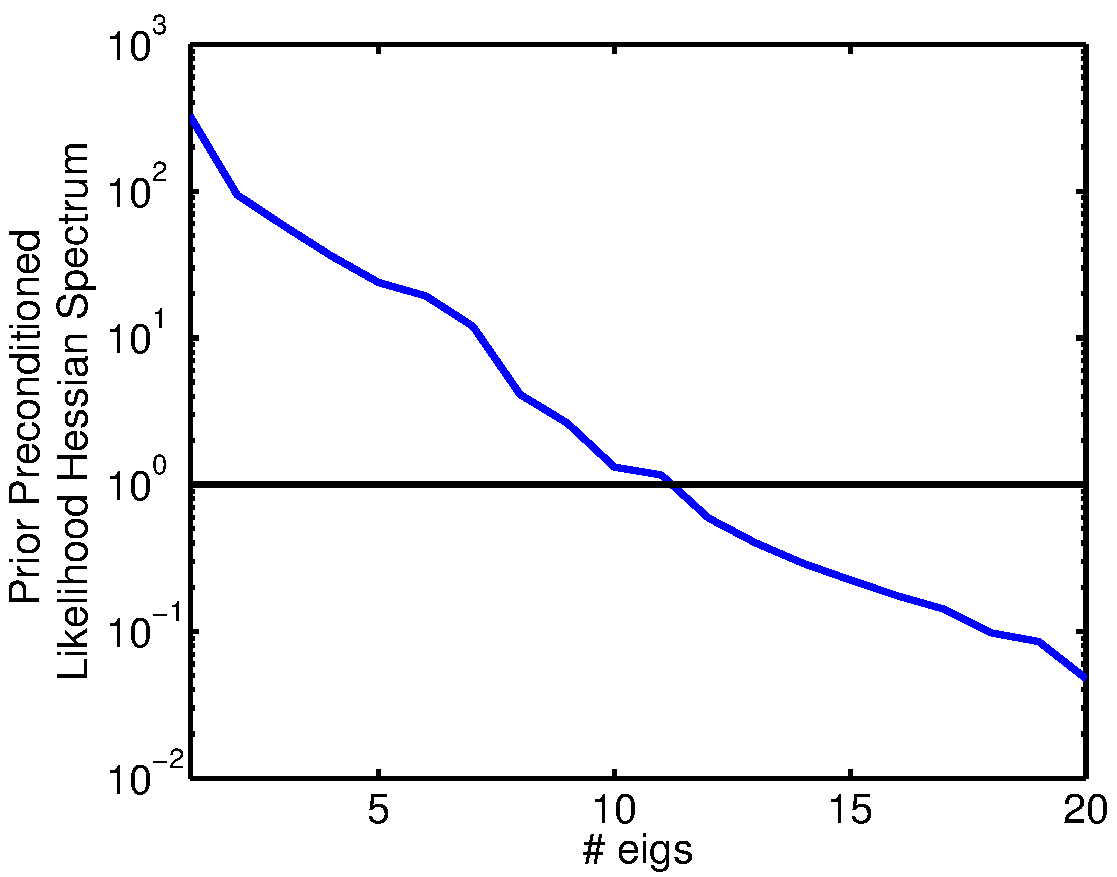
\includegraphics[width=0.35\textwidth]{extraplots/spectrum.pdf}
    \hspace{0.2in}
    \centering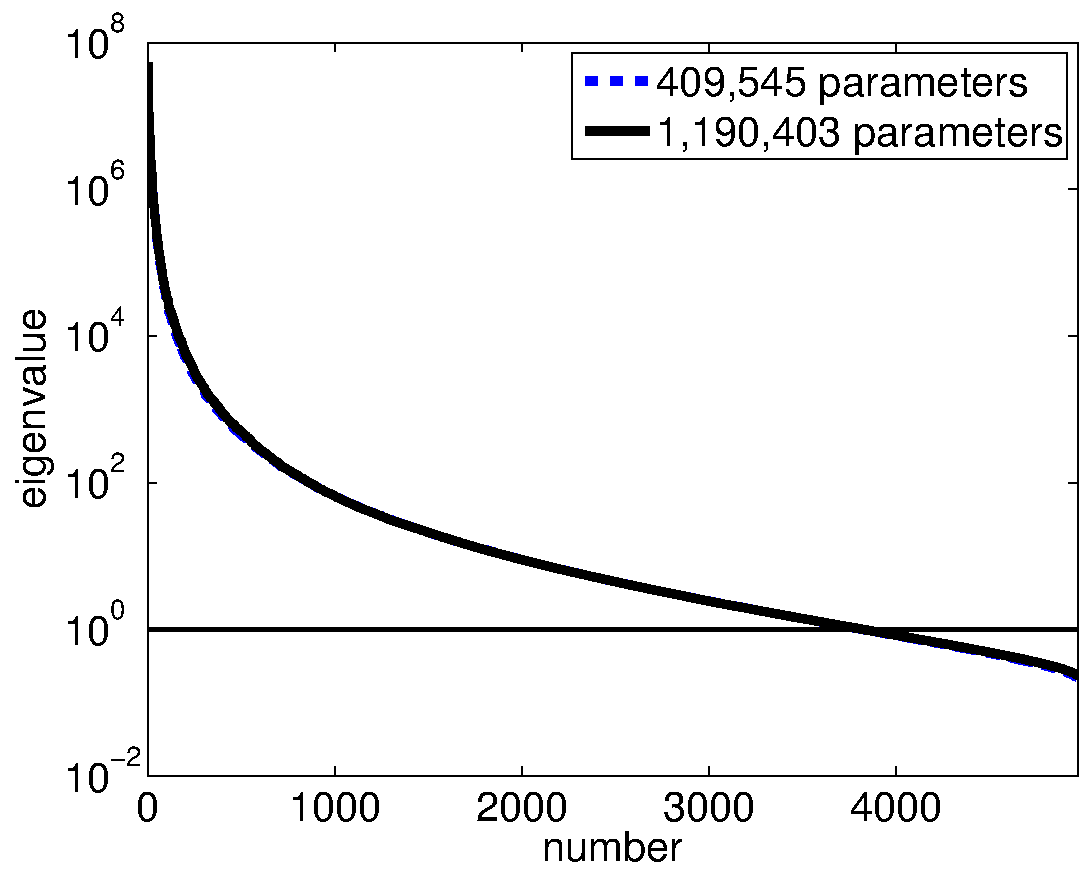
\includegraphics[width=0.35\textwidth]{extraplots/spec_ppmisfit_hess_coarseandfine_new.pdf}
  \end{figure}
  %
\end{itemize}
\end{frame}

%---------------------------------------------------------------------------------%
%---------------------------------------------------------------------------------%
%Story:
%
%Existing Hessian approximations are based on low-rank approximation
%methods, which require computing twice as many linearized forward or
%adjoint partial differential equation (PDE) solves as the numerical
%rank of the Hessian.
%
%These methods are inefficient when the numerical rank of the Hessian
%is large, as is the case in continental scale ice sheet inverse
%problems.
%
%Our goal is to take advantage of the off-diagonal low-rank structure
%of the Hessian and use {\note hierarchical matrix compression} to
%reduce the computational cost of solving the Bayesian ice sheet
%inverse problem.
%---------------------------------------------------------------------------------%
%---------------------------------------------------------------------------------%
\begin{frame}
 \frametitle{Exploiting the problem structure}
 \framesubtitle{Taking advantage of the parameter-to-observable mapping}
 \center

   \only<1>{
 \begin{tikzpicture}
 \fill[red!90,nearly transparent] (5,0) -- (7,.5) -- (3,.5) -- (1,0) -- cycle;
\draw [fill=red!40!white,opacity=1] (3,2.25) -- (3.5,2.25) -- (3.25,.25) -- cycle;
\draw [fill=red] (3.25,2.25) circle (.25cm and 0.07cm);
\draw (3.25,2.25) -- (2,3);
\draw [thick] (2,3) node[above]{sensitivities, $\frac{\partial u}{\partial\beta_j}$};
\draw[red,dashed] (7,.5) -- (3,.5) -- (1,0);
\draw [fill=blue!40!white,opacity=1] (4.25,.25) -- (4.5,2.25) -- (4.75,.25) -- cycle;
\draw [fill=blue] (4.5,.25) circle (.25cm and 0.07cm);
\draw (4.5,.25) -- (2,-.5);
\draw [thick] (2,-.5) node[below]{sensitivities, $\frac{\partial u_i}{\partial\beta}$};
\draw (1,0) -- (5,0) -- (5,2) -- (1,2) -- (1,0);
\draw  (5,2) -- (7,2.5) -- (3,2.5) -- (1,2);
\draw  (7,2.5) -- (7,.5) -- (5,0);
\draw  (5,2.25) -- (6,3) ;
\draw [thick] (6,3) node[above]{measurements, $\boldsymbol{d}$};
\draw[red]   (5.5,.25) -- (5.5,.125) ;
\draw  (5.5,.125) -- (5.5,-.5) ;
\draw [thick] (5.5,-.5) node[below]{parameter, $\beta(x)$};

\draw[dashed] (3,.5) -- (3,2);
\draw[blue,dashed] (3,2) -- (3,2.5);
\fill[blue!90,nearly transparent] (5,2) -- (7,2.5) -- (3,2.5) -- (1,2) -- cycle;
\end{tikzpicture}
   }
   \only<2>{
     \begin{center}
     	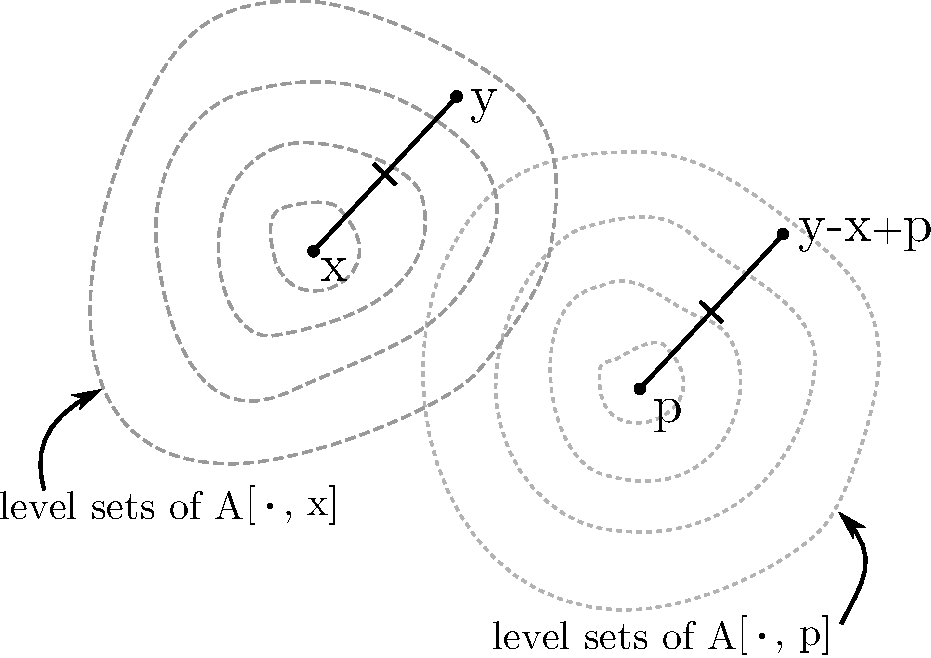
\includegraphics[width=0.6\columnwidth]{extraplots/translation_invariance_level_sets.pdf}
       %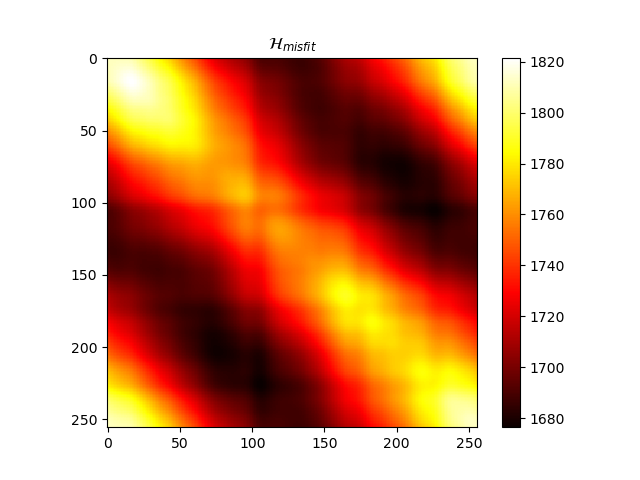
\includegraphics[width=0.6\columnwidth]{extraplots/Hess1_ordered.png}
     \end{center}
   }
	\only<3>{
	\begin{center}
		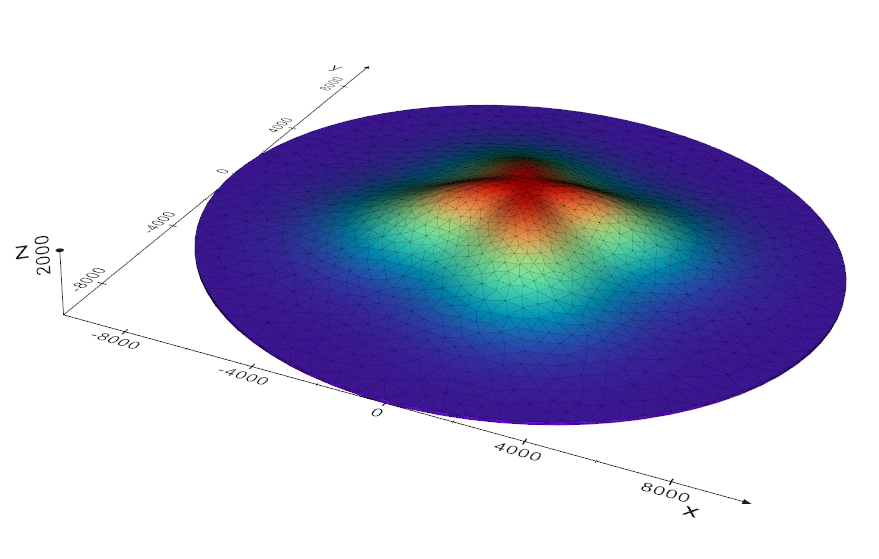
\includegraphics[width=0.6\columnwidth]{extraplots/Mesh_Height.png}
	\end{center}
	}
	\only<4>{
		\begin{center}
			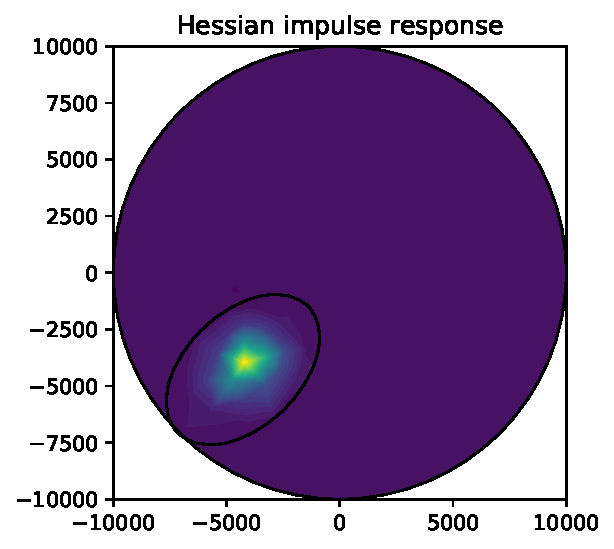
\includegraphics[width=0.45\columnwidth]{extraplots/ice_hessian_impulse_response_2.pdf}
		\end{center}
	}
	\only<5>{
	\begin{center}
		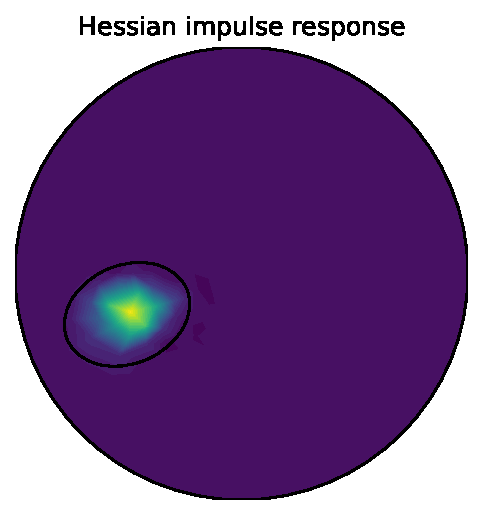
\includegraphics[width=0.45\columnwidth]{extraplots/ice_hessian_impulse_response_3.pdf}
	\end{center}
}
	\only<6>{
	\begin{center}
		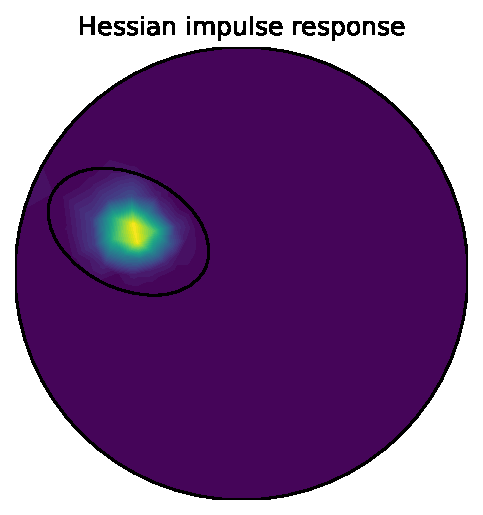
\includegraphics[width=0.45\columnwidth]{extraplots/ice_hessian_impulse_response_4.pdf}
	\end{center}
}
	\only<7>{
	\begin{center}
		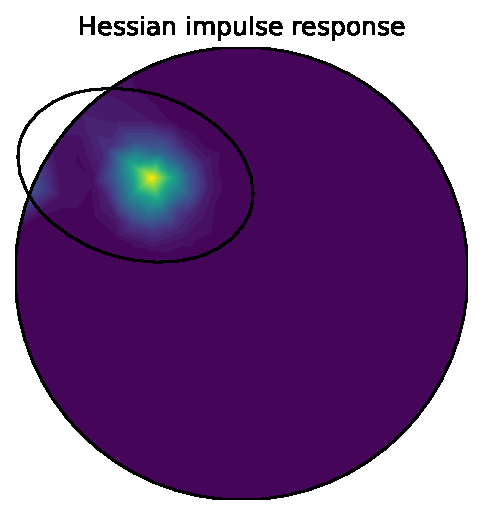
\includegraphics[width=0.45\columnwidth]{extraplots/ice_hessian_impulse_response_5.pdf}
	\end{center}
}
	\only<8>{
	\begin{center}
		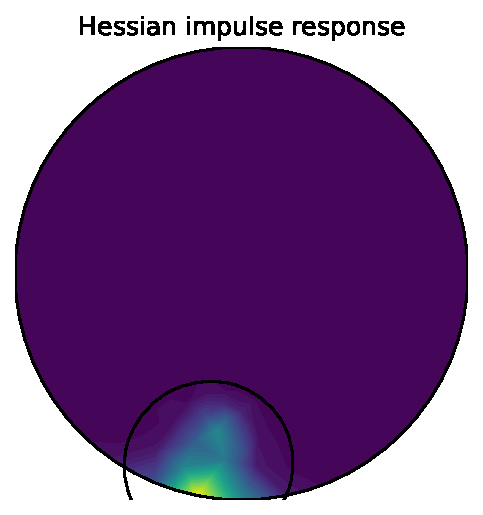
\includegraphics[width=0.45\columnwidth]{extraplots/ice_hessian_impulse_response_6.pdf}
	\end{center}
}
	\only<9>{
	\begin{center}
		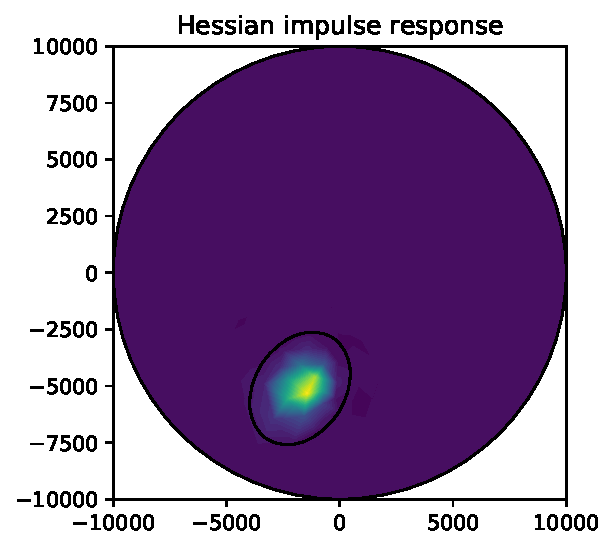
\includegraphics[width=0.45\columnwidth]{extraplots/ice_hessian_impulse_response_7.pdf}
	\end{center}
}
	\only<10>{
	\begin{center}
		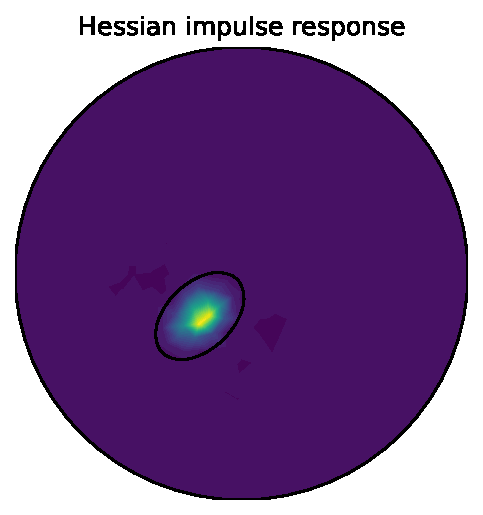
\includegraphics[width=0.45\columnwidth]{extraplots/ice_hessian_impulse_response_8.pdf}
	\end{center}
}
	\only<11>{
	\begin{center}
		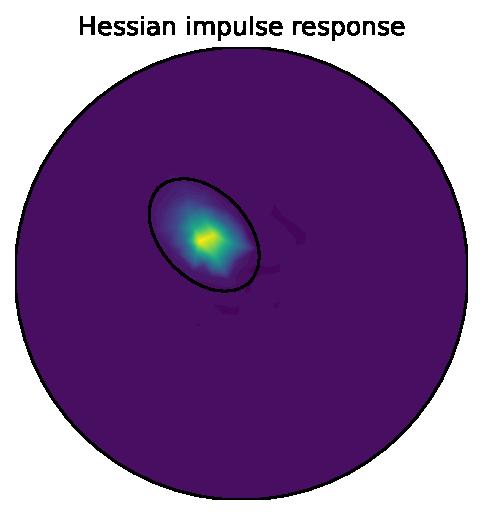
\includegraphics[width=0.45\columnwidth]{extraplots/ice_hessian_impulse_response_9.pdf}
	\end{center}
}
	\only<12>{
	\begin{center}
		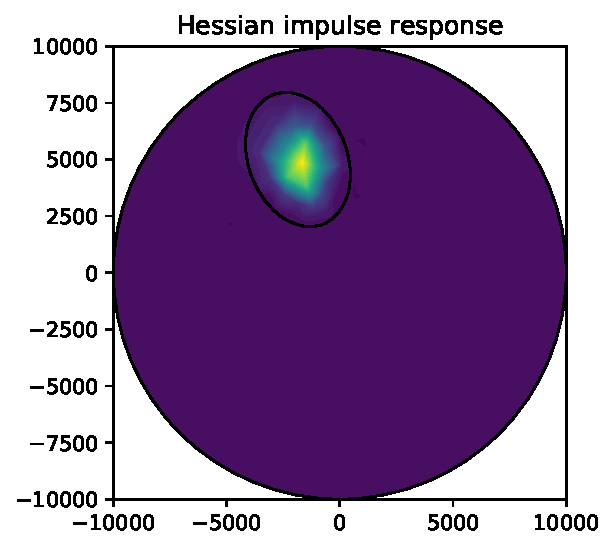
\includegraphics[width=0.45\columnwidth]{extraplots/ice_hessian_impulse_response_10.pdf}
	\end{center}
}
	\only<13>{
	\begin{center}
		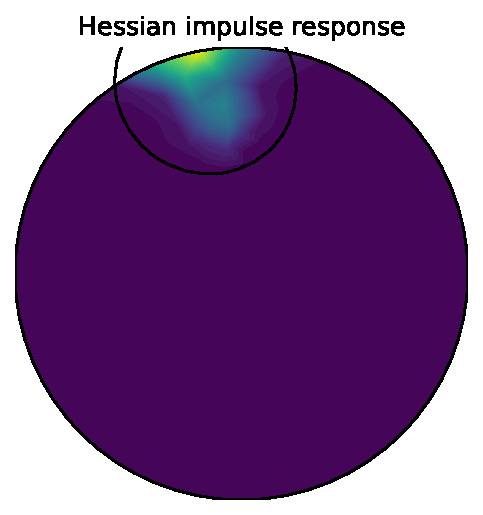
\includegraphics[width=0.45\columnwidth]{extraplots/ice_hessian_impulse_response_11.pdf}
	\end{center}
}
	\only<14>{
	\begin{center}
		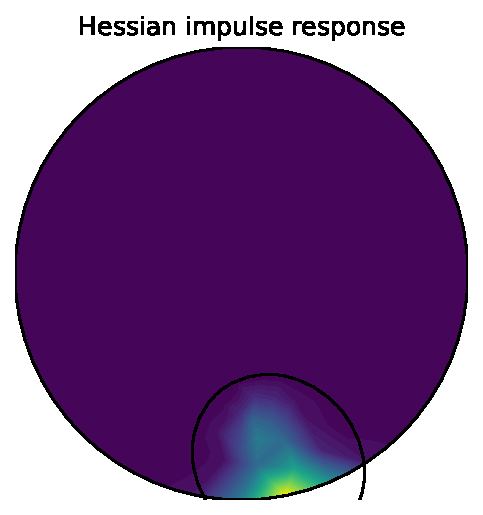
\includegraphics[width=0.45\columnwidth]{extraplots/ice_hessian_impulse_response_12.pdf}
	\end{center}
}
	\only<15>{
	\begin{center}
		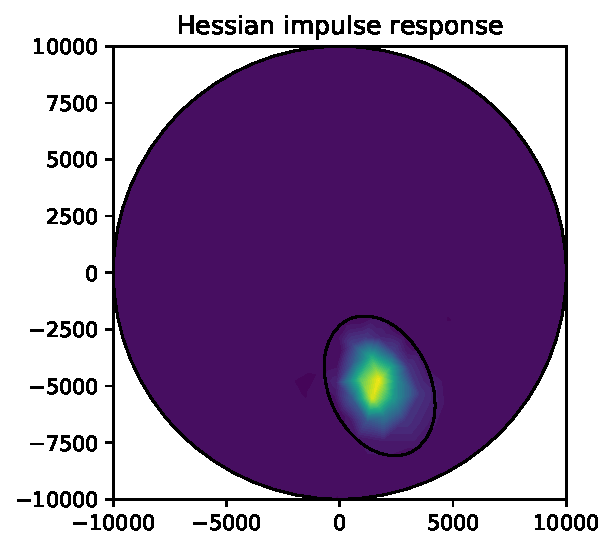
\includegraphics[width=0.45\columnwidth]{extraplots/ice_hessian_impulse_response_13.pdf}
	\end{center}
}
	\only<16>{
	\begin{center}
		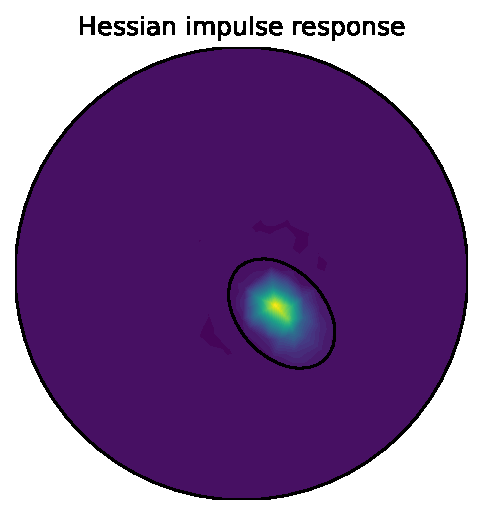
\includegraphics[width=0.45\columnwidth]{extraplots/ice_hessian_impulse_response_14.pdf}
	\end{center}
}
	\only<17>{
	\begin{center}
		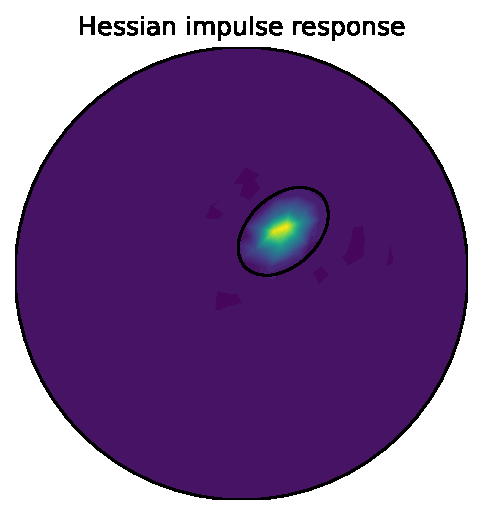
\includegraphics[width=0.45\columnwidth]{extraplots/ice_hessian_impulse_response_15.pdf}
	\end{center}
}
	\only<18>{
	\begin{center}
		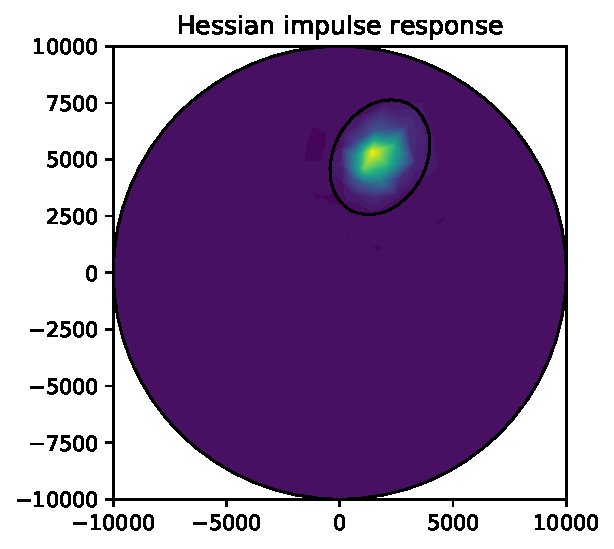
\includegraphics[width=0.45\columnwidth]{extraplots/ice_hessian_impulse_response_16.pdf}
	\end{center}
}
	\only<19>{
	\begin{center}
		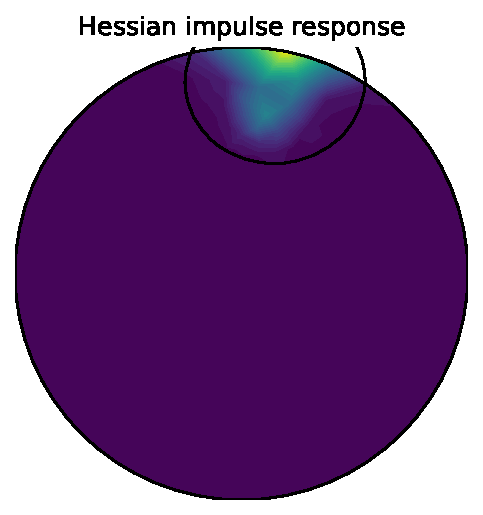
\includegraphics[width=0.45\columnwidth]{extraplots/ice_hessian_impulse_response_17.pdf}
	\end{center}
}
	\only<20>{
	\begin{center}
		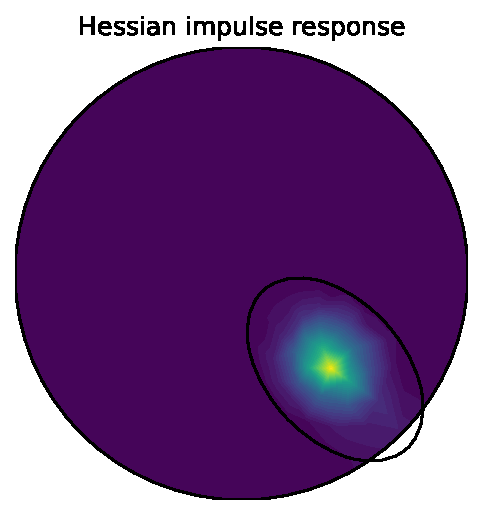
\includegraphics[width=0.45\columnwidth]{extraplots/ice_hessian_impulse_response_18.pdf}
	\end{center}
}
	\only<21>{
	\begin{center}
		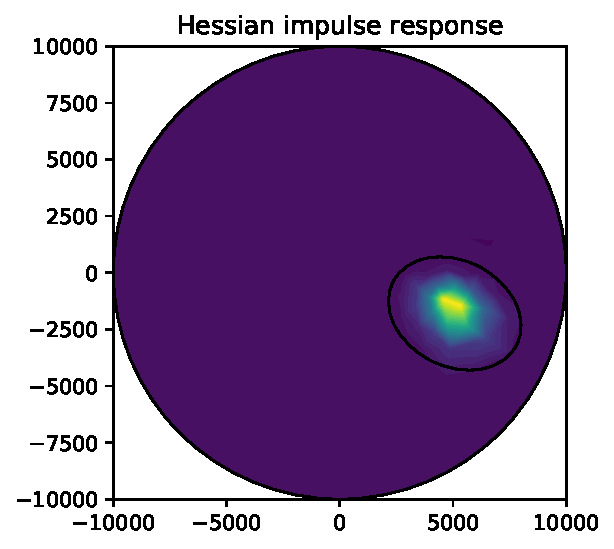
\includegraphics[width=0.45\columnwidth]{extraplots/ice_hessian_impulse_response_19.pdf}
	\end{center}
}
	\only<22>{
	\begin{center}
		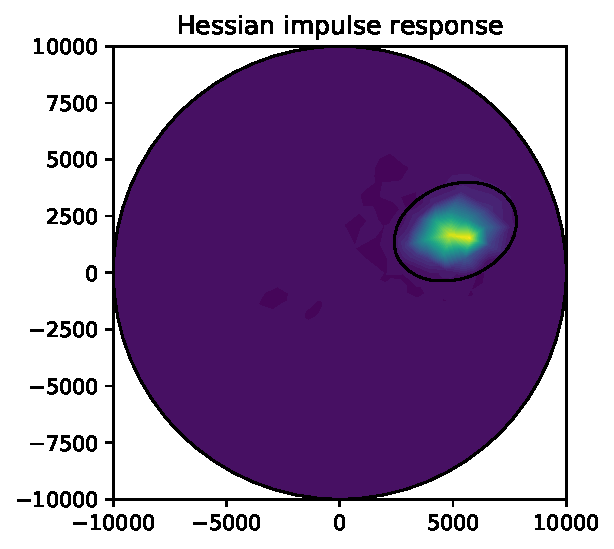
\includegraphics[width=0.45\columnwidth]{extraplots/ice_hessian_impulse_response_20.pdf}
	\end{center}
}
	\only<23>{
	\begin{center}
		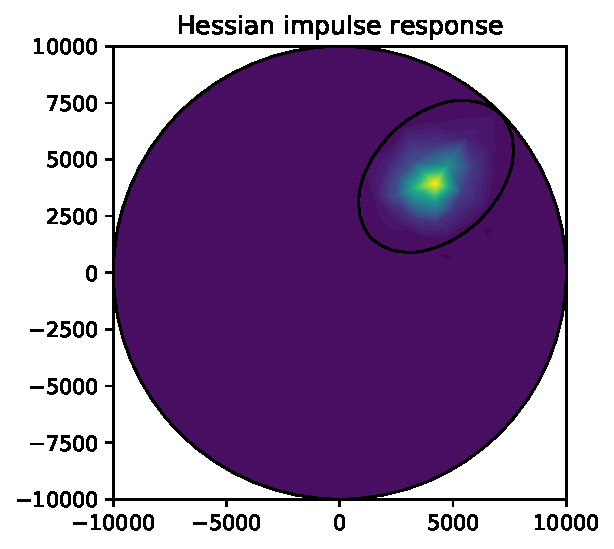
\includegraphics[width=0.45\columnwidth]{extraplots/ice_hessian_impulse_response_21.pdf}
	\end{center}
}

\begin{flushleft}Hessian properties:\end{flushleft}
\begin{itemize}
\item Local sensitivities
\item Local translation invariance
\end{itemize}
\end{frame}
%---------------------------------------------------------------------------------%
\begin{frame}
  \frametitle{Fast high-rank Hessian approximation for Bayesian ice
    sheet inverse problems}
      \begin{itemize}
      \item {\bf Stage 1: Hessian approximation via product-convolution
        approximation:}
        %leads to fast access to matrix entries, which
        %makes
        %the approximation well-suited for hierarchical matrix compression.
        %to reduce the computational cost of the
        %{$\mathcal{H}$-matrice compression, we first approximate the Hessian
        %  using a {\note product-convolution approximation approach} that
        %  takes advantage of the Hessian's local translation invariance.
        \begin{itemize}
        \item Compute {\bf the impulse responses} of the Hessian operator at
          many points by applying the operator to a small number of Dirac
          combs of point sources.
          %\item Within each Dirac comb, the point sources must be spaced
          %  sufficiently far apart so that the impulse responses to those
          %  point sources do not overlap with each other or with the boundary.
        \item Estimate the required spacing of point sources by applying the
          operator to a small number of constant, linear, and quadratic
          functions.
        \item Once computed, the impulse responses are interpolated to approximate arbitrary Hessian entries.
        \end{itemize}
      \item {\bf Stage 2: $\mathcal{H}$-matrix compression:}
        \begin{itemize}
        \item Convert the product-convolution Hessian approximation to
          hierarchical matrix format.
        \item Invert the compressed matrix using fast hierarchical matrix
          arithmetic.
        \end{itemize}

        \item {\bf Stage 3: Hessian-approximation via
          $\mathcal{H}$-matrix compression:}
          \begin{itemize}
            \item Use this approximation to precondition linear systems involving the Hessian (e.g., solve the Newton system to
              compute the MAP point) and/or draw samples from the
              posterior.
          \end{itemize}
      \end{itemize}
\end{frame}
%---------------------------------------------------------------------------------%
%---------------------------------------------------------------------------------%
\begin{frame}
\frametitle{Product-convolution approximation}
\framesubtitle{Batch of Hessian impulse responses}
\begin{center}
	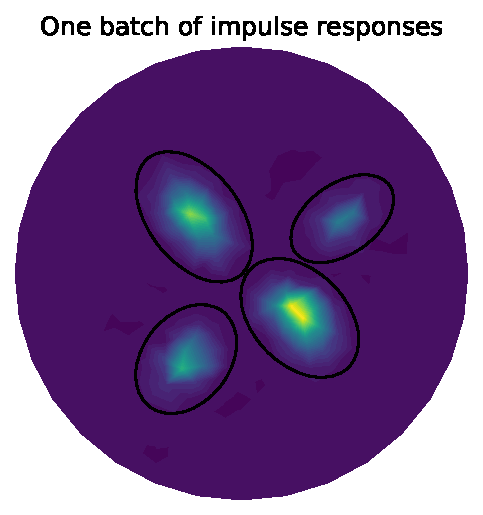
\includegraphics[width=0.45\columnwidth]{extraplots/ice_hessian_impulse_response_batch.pdf}
\end{center}
\end{frame}

\begin{frame}
	\frametitle{Product-convolution approximation}
	\framesubtitle{Weighting functions used for interpolation of impulse responses}
	\begin{center}
		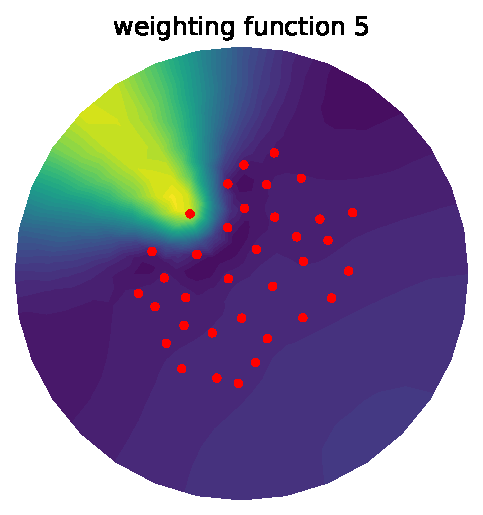
\includegraphics[width=0.3\columnwidth]{extraplots/ice_hessian_weighting_function_5.pdf}
		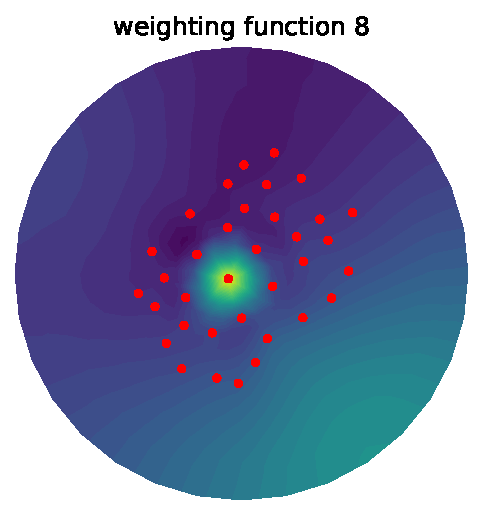
\includegraphics[width=0.3\columnwidth]{extraplots/ice_hessian_weighting_function_8.pdf}
		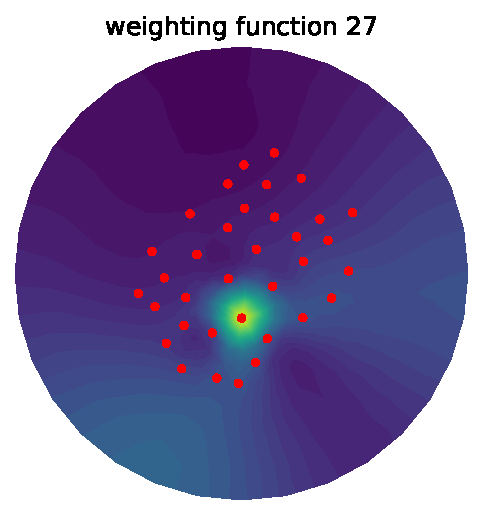
\includegraphics[width=0.3\columnwidth]{extraplots/ice_hessian_weighting_function_27.pdf}
	\end{center}
\end{frame}


\begin{frame}
	\frametitle{$\mathcal{H}$-matrix approximation}
	
	\begin{minipage}{0.49\textwidth} 
		\begin{itemize}
			\item Mesh points are 
			hierarchically partitioned into
			clusters by recursive hyperplane splitting.
			\item If two clusters are well separated, then the associated
			submatrix is low-rank.
		\end{itemize}
	\end{minipage}
	\begin{minipage}{0.49\textwidth}
		\begin{figure}[htb]
			\centering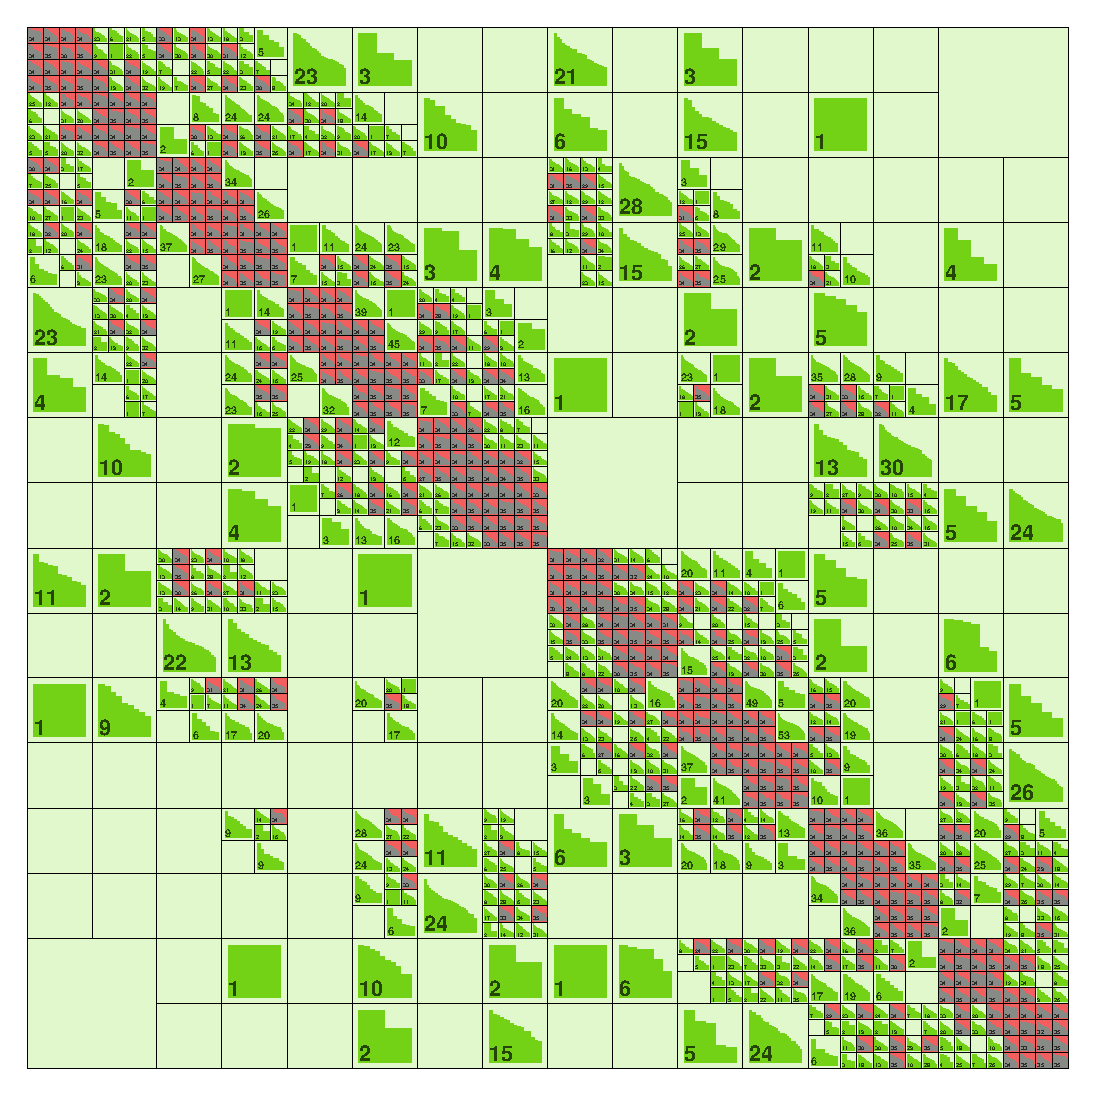
\includegraphics[width=0.5\textwidth]
			{extraplots/heat_inverse_problem_Hfull_hmatrix.eps}
		\end{figure}
		\begin{center}
			{\tiny $\mathcal{H}$-matrix structure of a diffusion
				inverse problem Hessian \\}
		\end{center}
	\end{minipage}
	
	\begin{itemize}
		\item 
		$\mathcal{H}$-matrix operations are fast: $\mathcal{O}\left(n\,\log\left(n\right)\right)$
		matrix-vector product, $\mathcal{O}\left(n\,\log^{2}\left(n\right)\right)$
		LU factorization.
	\end{itemize}
	
	\scriptsize{
		\begin{itemize}
%			\item[]    Details in:
%			\item[]    N. Halko, P.G. Martinsson, J Tropp.
%			{\em Finding structure with randomness: Probabilistic
%				algorithms for constructing approximate matrix
%				decompositions}, SIAM review, 2011.
			\item[]  R. Kriemann.
			{\em HLIBpro user manual}, Max-Planck-Institute
			for Mathematics in the Sciences, Leipzig, 2008
			\item[]   J. Ballani, D. Kressner.
			{\em Matrices with Hierarchical Low-Rank Structures},
			Exploiting Hidden Structure in Matrix Compuations:
			Algorithms and Applications, 2016
		\end{itemize}
	}
	
\end{frame}
\begin{frame}
	\frametitle{Hessian approximation is a good preconditioner}
	\begin{center}
		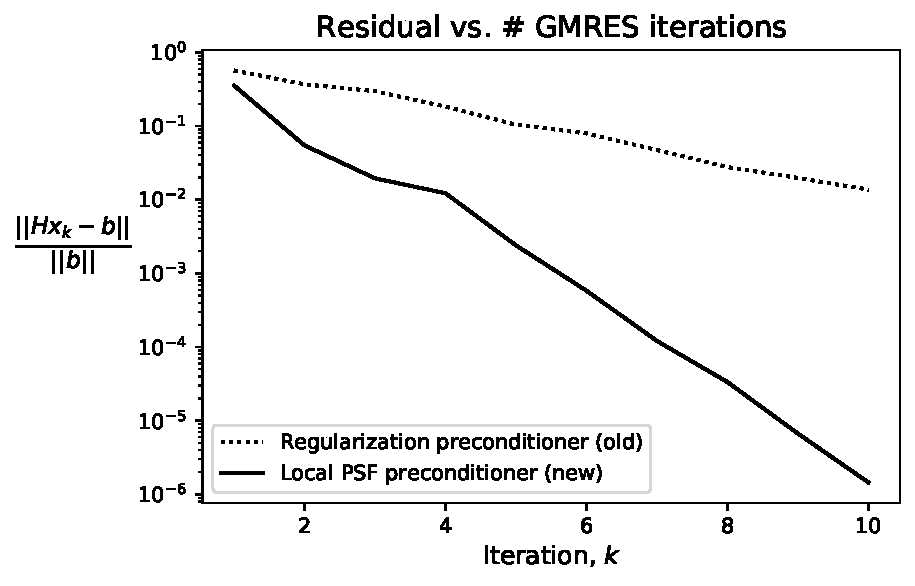
\includegraphics[width=0.75\columnwidth]{extraplots/ice_gmres_convergence.pdf}
	\end{center}
\begin{center}
	H-matrix compressed Hessian approximation, used as a preconditioner, leads to fast Krylov method convergence.
\end{center}
\end{frame}
%--------------------------------------------------------------------------
\begin{frame}
  \frametitle{Summary}

  \begin{itemize}
  \item Hessians in inverse problems governed by
    partial differential equations are essential for
    efficient, dimension-independent methods for both
    \begin{itemize}
    \item Newton solution of deterministic inverse problems (i.e., for
      computing the MAP point);
      \vspace{0.05in}
    \item Markov chain Monte Carlo sampling to characterize the
      posterior.
    \end{itemize}
    \vspace{0.05in}
  \item Low-rank approximations of the Hessian become
    prohibitive as the data becomes more informative (as is the case
    for ice sheet inverse problems).
    \vspace{0.05in}
  \item Hierarchical matrix representations promise a more efficient
    Hessian approximation.
  \end{itemize}
    \vspace{0.2in}
  \begin{itemize}
  \item [] \scriptsize{Details in: N. Alger, T. Hartland, N. Petra,
    and O. Ghattas. {\em Fast matrix-free approximation of smoothly
      varying blur operators, with application to Hessians in
      PDE-constrained inverse problems with highly informative data},
    In preparation.}
  \end{itemize}
\end{frame}
\end{document}
